\subsection{ANTICOMMUTATIVE ALGEBRAS AND ALTERNATING ALGEBRAS}

DEFINITION 7. A graded A-algebra E of type Z is called anticommutative if for all non-zero homogeneous elements x, y of E

\[
x y = (- 1) ^ {\deg (x) \deg (y)} y x.\tag{36}
\]

The algebra \(\mathbf{E}\) is called alternating if it is anticommutative and also \(x^{2} = 0\) for every homogeneous element \(x\in \mathbf{E}\) of odd degree.

Remarks. (1) Let \(\mathbf{E}^{+}\) be the graded subalgebra of \(\mathbf{E}\) the direct sum of the \(\mathrm{E}_{2n}\) ( \(n \in \mathbf{Z}\) ); it follows from Definition 7 that if \(\mathbf{E}\) is anticommutative, \(\mathbf{E}^{+}\) is a subalgebra contained in the centre of \(\mathbf{E}\) (and hence commutative).

\begin{enumerate}
\def\labelenumi{(\arabic{enumi})}
\setcounter{enumi}{1}
\item
  Suppose that 2 is not a divisor of 0 in E; then if E is anticommutative E is alternating, since for \(x \in E\) homogeneous and of odd degree, \(x^{2} = -x^{2}\) by (36), whence \(2x^{2} = 0\) and \(x^{2} = 0\) by virtue of the hypothesis.
\item
  We shall study in detail in § 7 important examples of alternating algebras.
\end{enumerate}

Lemma 4. Let E be a graded algebra of type Z and S a set of homogeneous elements \(\neq0\) ; the set F of elements of E all of whose homogeneous components \(x\neq0\) satisfy relation (36) for all \(y\in S\) is a graded subalgebra of E.

It suffices to note that: (1) if \(x'\) , \(x''\) are two homogeneous elements of the same degree \(p\) , \(y\) a homogeneous element of degree \(q\) and \(x'y = (-1)^{pq}yx'\) , \(x''y = (-1)^{pq}yx''\) , then also \((x' + x'')y = (-1)^{pq}y(x' + x'')\) ; (2) if \(x'\) , \(x''\) are two homogeneous elements of respective degrees \(p'\) , \(p'', y\) a homogeneous element of degree \(q\) and \(x'y = (-1)^{p'q}yx'\) , \(x''y = (-1)^{p''q}yx''\) , then

\[
(x ^ {\prime} x ^ {\prime \prime}) y = (- 1) ^ {(p ^ {\prime} + p ^ {\prime \prime}) q} y (x ^ {\prime} x ^ {\prime \prime}).
\]

PROPOSITION 13. Let E be a graded A-algebra of type Z and S a generating system of the algebra E consisting of homogeneous elements \(\neq0\) ; for E to be anticommutative (resp. alternating), it is necessary and sufficient that (36) hold for all \(x\in S\) and \(y\in S\) (resp. that this condition holds and further that \(x^{2}=0\) for all x homogeneous of odd degree belonging to S).

We consider first the case of anticommutative algebras. By Lemma 4, the subalgebra F consisting of the elements all of whose homogeneous components \(x \neq 0\) satisfy (36) for all \(y \in S\) , contains all the elements of S and hence F = E. If now \(F'\) is similarly the subalgebra of E consisting of the elements all of whose homogeneous components \(x \neq 0\) satisfy (36) for every homogeneous element \(y \neq 0\) , it follows from the above that \(F'\) contains all the elements of S and hence \(F' = E\) , which completes the proof of the proposition in this case.

To prove the proposition in the case of alternating algebras, it can be assumed that E is already anticommutative; it is then immediate that every homogeneous element of odd degree in E is of the form \(\sum_{i} z_{i} x_{i}\) , where \(z_{i} \in E^{+}\) and \(x_{i} \in S\) is of odd degree (using the fact that \(E^{+}\) is contained in the centre of E); it follows that \(\left(\sum_{i} z_{i} x_{i}\right)^{2} = \sum_{i} z_{i}^{2} x_{i}^{2} + \sum_{i < j} z_{i} z_{j} (x_{i} x_{j} + x_{j} x_{i}) = 0\) since \(x_{i}^{2} = 0\) by hypothesis and \(x_{i} x_{j} + x_{j} x_{i} = 0\) by (36).

PROPOSITION 14. Let E and F be two graded A-algebras of type Z, both anticommutative (resp. alternating). Then the skew tensor product \(\mathbf{E}^{\mathbf{g}}\otimes_{\mathbf{A}}\mathbf{F}\) (no. 7) is an anticommutative (resp. alternating) algebra.

A generating system of \(E^{g} \otimes_{A} F\) consists of the \(x \otimes y\) , where x (resp. y) is a homogeneous element \(\neq 0\) of E (resp. F). Consider two such elements \(x \otimes y\) , \(x' \otimes y'\) , with \(\deg(x) = p\) , \(\deg(y) = q\) , \(\deg(x') = p'\) , \(\deg(y') = q'\) , so that \(x \otimes y\) is of degree \(p + q\) and \(x' \otimes y'\) of degree \(p' + q'\) . Then by definition (no. 7, formula (27)) and by virtue of (36),

\[
(x \otimes y) (x ^ {\prime} \otimes y ^ {\prime}) = (- 1) ^ {q p ^ {\prime}} (x x ^ {\prime}) \otimes (y y ^ {\prime})
\]

\[
\begin{array}{r l} (x ^ {\prime} \otimes y ^ {\prime}) (x \otimes y) & = (- 1) ^ {p q ^ {\prime}} (x ^ {\prime} x) \otimes (y ^ {\prime} y) \\ & = (- 1) ^ {p q ^ {\prime} + p p ^ {\prime} + q q ^ {\prime}} (x x ^ {\prime}) \otimes (y y ^ {\prime}) \end{array}
\]

and the criterion of Proposition 13 shows that \(\mathbf{E}^{\mathbf{g}}\otimes_{\mathbf{A}}\mathbf{F}\) is anticommutative since \(pq' + p p' + qq' - q p' \equiv (p + q)(p' + q')\) (mod. 2). If further E and F are alternating and \(p + q\) is odd, one of the numbers \(p, q\) is necessarily odd, hence \((x \otimes y)^2 = \pm (x^2) \otimes (y^2) = 0\) and Proposition 13 shows that \(E^g \otimes_A F\) is alternating.

COROLLARY. Let E be an anticommutative (resp. alternating) graded A-algebra of type Z. Then for every ring homomorphism \(\rho: \mathrm{A} \to \mathrm{B}\) , the graded B-algebra \(\rho^{*}(\mathrm{E})\) (no. 8, Remark 2) is anticommutative (resp. alternating).

The ring B with the trivial graduation can be considered as an alternating A-algebra and \(\rho^{*}(\mathbf{E}) = \mathbf{E}^{\mathfrak{g}}\otimes_{\mathbf{A}}\mathbf{B}\) , hence Proposition 14 can be applied.

Remark. Let E be an anticommutative graded A-algebra of type Z. Then the A-linear mapping of \(E \otimes_{A} E\) into E defined by multiplication of E (§1, no. 3) is a homomorphism of the graded A-algebra \(E^{g} \otimes_{A} E\) into E, for in the notation of Proposition 14, in the algebra E,

\[
(x y) (x ^ {\prime} y ^ {\prime}) = (- 1) ^ {q p ^ {\prime}} (x x ^ {\prime}) (y y ^ {\prime}).
\]

\section{TENSOR ALGEBRA, TENSORS}

\subsection{DEFINITION OF THE TENSOR ALGEBRA OF A MODULE}

Let A be a commutative ring and M an A-module. For every integer \(n \geqslant 0\) , the A-module the tensor product of n modules equal to M (also called the n-th tensor power of M) is denoted by \(\bigotimes^{n} M\) , or \(M^{\otimes n}\) , or \(T^{n}(M)\) , or \(T_{A}^{n}(M)\) , or \(\operatorname{Tens}^{n}(M)\) ; then \(T^{1}(M) = M\) ; also we write \(T^{0}(M) = A\) . The A-module the direct sum \(\bigoplus_{n \geqslant 0} T^{n}(M)\) is denoted by \(T(M)\) or \(\operatorname{Tens}(M)\) . We shall define a graded A-algebra structure of type N on \(T(M)\) , by defining for every ordered pair of integers \(p \geqslant 0\) , \(q \geqslant 0\) , an A-linear mapping

\[
m _ {p q} \colon \mathsf {T} ^ {p} (\mathbf {M}) \otimes_ {\mathbf {A}} \mathsf {T} ^ {q} (\mathbf {M}) \rightarrow \mathsf {T} ^ {p + q} (\mathbf {M})
\]

(§ 3, no. 1, Remark). For \(p > 0\) and \(q > 0\) , \(m_{pq}\) is the associativity isomorphism (II, § 3, no. 9) and, when \(p = 0\) (resp. \(q = 0\) ), \(m_{0,q}\) is the canonical isomorphism of \(A \otimes_A T^q(M)\) onto \(T^q(M)\) (resp. \(m_{p,0}\) is the canonical isomorphism of \(T^p(M) \otimes_A A\) onto \(T^p(M)\)) (II, § 3, no. 4, Proposition 4). Then, for \(x_t \in M\) , \(\alpha \in A\) ,

\[
\left\{ \begin{array}{r l} (x _ {1} \otimes \dots \otimes x _ {p}) \cdot (x _ {p + 1} \otimes \dots \otimes x _ {p + q}) & \\ = x _ {1} \otimes \dots \otimes x _ {p} \otimes x _ {p + 1} \otimes \dots \otimes x _ {p + q} \\ \alpha \cdot (x _ {1} \otimes \dots \otimes x _ {p}) = \alpha (x _ {1} \otimes \dots \otimes x _ {p}). \end{array} \right.\tag{1}
\]

It is immediate that the multiplication thus defined on \(\mathsf{T}(\mathbf{M})\) is associative and admits as unit element the unit element \(1\) of \(\mathbf{A} = \mathsf{T}^0 (\mathbf{M})\) .

DEFINITION 1. For every module M over a commutative ring A, the tensor algebra of M, denoted by T(M), or Tens(M), or \(\mathsf{T}_{\mathbf{A}}(\mathbf{M})\) , is the algebra \(\bigoplus_{n\geqslant 0}\mathsf{T}^n (\mathbf{M})\) with the multiplication defined in (1). The canonical injection \(\phi :\mathsf{T}^{1}(\mathbf{M})\to \mathsf{T}(\mathbf{M})\) (II, § 1, no. 12) (also denoted by \(\phi_{\mathbf{M}}\) ) is called the canonical injection of M into T(M).

PROPOSITION 1. Let E be a (unital) A-algebra and \(f:M\to E\) an A-linear mapping. There exists one and only one A-algebra homomorphism \(g:T(M)\to E\) such that \(f=g\circ\phi\) .

In other words, \((\mathsf{T}(\mathbf{M}), \phi)\) is a solution of the universal mapping problem (Set Theory, IV, §3, no. 1), where \(\Sigma\) is the species of A-algebra structure, the \(\alpha\) -mappings being the A-linear mappings from the module M to an A-algebra. Observe that here there is no question of a graduation on \(\mathsf{T}(\mathbf{M})\) .

For every finite family \((x_{i})_{1\leqslant i\leqslant n}\) of n elements of M, by definition of the product in T(M), \(x_{1}\otimes x_{2}\otimes\cdots\otimes x_{n}=\phi(x_{1})\phi(x_{2})\ldots\phi(x_{n})\) ; then necessarily \(g(x_{1}\otimes x_{2}\otimes\cdots\otimes x_{n})=f(x_{1})f(x_{2})\ldots f(x_{n})\) for \(n\geqslant1\) and \(g(\alpha)=\alpha e\) (if e is the unit element of E) for \(\alpha\in A\) , which proves the uniqueness of g. Conversely, note that, for all n\textgreater0, the mapping

\[
(x _ {1}, \dots , x _ {n}) \mapsto f (x _ {1}) f (x _ {2}) \dots f (x _ {n})
\]

of \(\mathbf{M}^n\) into \(\mathbf{E}\) is A-multilinear; hence there corresponds to it an A-linear mapping \(g_n: \mathsf{T}^n(\mathbf{M}) \to \mathbf{E}\) such that

\[
g \left(x _ {1} \otimes x _ {2} \otimes \dots \otimes x _ {n}\right) = f \left(x _ {1}\right) f \left(x _ {2}\right) \dots f \left(x _ {n}\right).\tag{2}
\]

Also we define the mapping \(g_0 \colon \mathsf{T}^0(\mathbf{M}) \to \mathbf{E}\) as equal to \(\eta_{\mathbf{E}}\) (§ 1, no. 3), in other words \(g_0(\alpha) = \alpha e\) for \(\alpha \in \mathbf{A}\) . Let \(g\) be the unique A-linear mapping of \(\mathsf{T}(\mathbf{M})\) into \(\mathbf{E}\) whose restriction to \(\mathsf{T}^n(\mathbf{M})\) is \(g_n\) ( \(n \geqslant 0\) ); it is immediate that \(g \circ \phi = g_1 = f\) and it remains to verify that \(g\) is an A-algebra homomorphism. By construction \(g(1) = e\) and it suffices by linearity to show that \(g(uv) = g(u)g(v)\) for \(u \in \mathsf{T}^p(\mathbf{M})\) and \(v \in \mathsf{T}^q(\mathbf{M})\) ( \(p > 0, q > 0\) ); now it follows from formulae (1) and (2) that this relation is true when \(u = x_1 \otimes x_2 \otimes \cdots \otimes x_p\) and \(v = x_{p+1} \otimes \cdots \otimes x_{p+q}\) (where the \(x_i\) belong to \(\mathbf{M}\) ). It is therefore true for \(u \in \mathsf{T}^p(\mathbf{M})\) and \(v \in \mathsf{T}^q(\mathbf{M})\) by linearity.

Remark. Suppose that \(\mathbf{E}\) is a graded A-algebra of type \(\mathbf{Z}\) , with graduation \((\mathbf{E}_n)\) , and suppose also that

\[
f (\mathbf {M}) \subset \mathrm{E} _ {1}.\tag{3}
\]

Then it follows from (2) that \(g(\mathsf{T}^p (\mathbf{M})) \subset \mathrm{E}_p\) for all \(p \geqslant 0\) and hence \(g\) is a graded algebra homomorphism.

\subsection{FUNCTORIAL PROPERTIES OF THE TENSOR ALGEBRA}

PROPOSITION 2. Let A be a commutative ring, M and N two A-modules and

\[
u: \mathbf {M} \rightarrow \mathbf {N}
\]

an A-linear mapping. There exists one and only one A-algebra homomorphism

\[
u ^ {\prime}: \mathsf {T} (\mathbf {M}) \rightarrow \mathsf {T} (\mathbf {N})
\]

such that the diagram

\pandocbounded{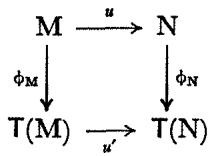
\includegraphics[keepaspectratio]{images/part003_fafbfb88.jpg}}

is commutative. Further, \(u'\) is a graded algebra homomorphism.

The existence and uniqueness of \(u'\) follow from no. 1, Proposition 1, applied to the algebra \(T(N)\) and the linear mapping \(\phi_N \circ u: M \to T(N)\) ; as

\[
u (\mathbf {M}) \subset \mathsf {T} ^ {1} (\mathbf {N}) = \mathbf {N},
\]

the fact that \(u'\) is a graded algebra homomorphism follows from the Remark of no. 1.

The homomorphism \(u'\) of Proposition 2 will henceforth be denoted by \(T(u)\) . If \(P\) is an A-module and \(v: N \to P\) an A-linear mapping, then

\[
\mathsf {T} (v \circ u) = \mathsf {T} (v) \circ \mathsf {T} (u)\tag{4}
\]

for \(\mathsf{T}(v)\circ \mathsf{T}(u)\) is an algebra homomorphism rendering commutative the diagram

\pandocbounded{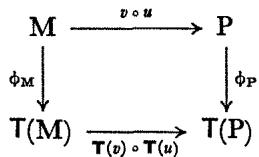
\includegraphics[keepaspectratio]{images/part003_f792dba1.jpg}}

\(\mathsf{T}(u)\) is sometimes called the canonical extension of u to \(\mathsf{T}(\mathbf{M})\) (which contains \(\mathbf{M} = \mathsf{T}^1(\mathbf{M})\) ). Note that the restriction \(\mathsf{T}^n(u): \mathsf{T}^n(\mathbf{M}) \to \mathsf{T}^n(\mathbf{N})\) is just the linear mapping \(u^{\otimes n} = u \otimes u \otimes \cdots \otimes u\) (n times), for

\[
\mathsf {T} ^ {n} (u) \left(x _ {1} \otimes \dots \otimes x _ {n}\right) = u \left(x _ {1}\right) \otimes \dots \otimes u \left(x _ {n}\right)
\]

since \(\mathsf{T}(u)\) is an algebra homomorphism and \(\mathsf{T}^{1}(u)=u\) ; the restriction \(\mathsf{T}^{0}(u)\) to A is the identity mapping. \(\mathsf{T}^{n}(u)\) is called the n-th tensor power of u.

PROPOSITION 3. If \(u: \mathbf{M} \to \mathbf{N}\) is a surjective A-linear mapping, the homomorphism \(\mathsf{T}(u): \mathsf{T}(\mathbf{M}) \to \mathsf{T}(\mathbf{N})\) is surjective and its kernel is the two-sided ideal of \(\mathsf{T}(\mathbf{M})\) generated by the kernel \(\mathbf{P} \subset \mathbf{M} \subset \mathsf{T}(\mathbf{M})\) of \(u\) .

\(T^{0}(u):T^{0}(M)\rightarrow T^{0}(N)\) is bijective and for every integer n\textgreater0,

\[
\mathbf {T} ^ {n} (u): \mathbf {T} ^ {n} (\mathbf {M}) \rightarrow \mathbf {T} ^ {n} (\mathbf {N})
\]

is surjective, as is seen by induction on \(n\) using II, § 3, no. 6, Proposition 6; the latter proposition also shows, by induction on \(n\) , that the kernel \(\mathfrak{S}_n\) of \(\mathsf{T}^n(u)\) is the submodule of \(\mathsf{T}^n(\mathbf{M})\) generated by the products

\[
x _ {1} \otimes x _ {2} \otimes \dots \otimes x _ {n}
\]

where at least one of the \(x_{i}\) belongs to \(\mathbf{P}\) . This shows that the kernel \(\mathfrak{S} = \bigoplus_{n\geqslant 1}\mathfrak{S}_n\) of \(\mathsf{T}(u)\) is the two-sided ideal generated by \(\mathbf{P}\) in \(\mathsf{T}(\mathbf{M})\) .

If \(u: \mathbf{M} \to \mathbf{N}\) is an injective linear mapping, it is not always true that \(\mathbf{T}(u)\) is an injective mapping (Exercise 1). However, this is true when \(u\) is an injection such that \(u(\mathbf{M})\) is a direct factor of \(\mathbf{N}\) , for then there exists a linear mapping \(v: \mathbf{N} \to \mathbf{M}\) such that \(v \circ u\) is the identity mapping on \(\mathbf{M}\) and therefore

\[
\mathsf {T} (v \circ u) = \mathsf {T} (v) \circ \mathsf {T} (u)
\]

is the identity mapping on \(\mathsf{T}(\mathbf{M})\) , hence \(\mathsf{T}(u)\) is injective and its image (isomorphic to \(\mathsf{T}(\mathbf{M})\) ) is a direct factor of \(\mathsf{T}(\mathbf{N})\) (II, §1, no. 9, Proposition 15). More precisely:

PROPOSITION 4. Let N and P be two submodules of an A-module M such that their sum \(N + P\) is a direct factor in M and their intersection \(N \cap P\) is a direct factor in N and in P. Then the homomorphisms \(\mathsf{T}(\mathbf{N}) \to \mathsf{T}(\mathbf{M})\) , \(\mathsf{T}(\mathbf{P}) \to \mathsf{T}(\mathbf{M})\) and

\[
\mathsf {T} (\mathbf {N} \cap \mathbf {P}) \rightarrow \mathsf {T} (\mathbf {M}),
\]

canonical extensions of the canonical injections, are injective; if \(\mathsf{T}(\mathbf{N})\) , \(\mathsf{T}(\mathbf{P})\) and \(\mathsf{T}(\mathbf{N} \cap \mathbf{P})\) are identified with subalgebras of \(\mathsf{T}(\mathbf{M})\) by means of these homomorphisms, then

\[
\mathsf {T} (\mathbf {N} \cap \mathbf {P}) = \mathsf {T} (\mathbf {N}) \cap \mathsf {T} (\mathbf {P}).\tag{5}
\]

By hypothesis, there exist submodules \(N' \subset N\) and \(P' \subset P\) such that \(N = N' \oplus (N \cap P)\) , \(P = P' \oplus (N \cap P)\) ; then

\[
\mathbf {N} + \mathbf {P} = \mathbf {N} ^ {\prime} \oplus \mathbf {P} ^ {\prime} \oplus (\mathbf {N} \cap \mathbf {P})
\]

and there exists by hypothesis a submodule \(M'\) of M such that

\[
\begin{array}{c} \mathbf {M} = \mathbf {M} ^ {\prime} \oplus (\mathbf {N} + \mathbf {P}) = \mathbf {M} ^ {\prime} \oplus \mathbf {N} ^ {\prime} \oplus \mathbf {P} ^ {\prime} \oplus (\mathbf {N} \cap \mathbf {P}) \\ = \mathbf {M} ^ {\prime} \oplus \mathbf {P} ^ {\prime} \oplus \mathbf {N} = \mathbf {M} ^ {\prime} \oplus \mathbf {N} ^ {\prime} \oplus \mathbf {P}. \end{array}
\]

In particular, \(N + P\) , N, P and \(N \cap P\) are direct factors in M, which implies, as has been seen above, that the canonical homomorphisms

\[
\begin{array}{l} \mathsf {T} (\mathbf {N} + \mathbf {P}) \to \mathsf {T} (\mathbf {M}), \qquad \mathsf {T} (\mathbf {N}) \to \mathsf {T} (\mathbf {M}), \\ \mathsf {T} (\mathbf {P}) \to \mathsf {T} (\mathbf {M}), \qquad \mathsf {T} (\mathbf {N} \cap \mathbf {P}) \to \mathsf {T} (\mathbf {M}) \end{array}
\]

are injective. The three algebras \(\mathsf{T}(\mathbf{N})\) , \(\mathsf{T}(\mathbf{P})\) and \(\mathsf{T}(\mathbf{N} \cap \mathbf{P})\) are thus identified with subalgebras of \(\mathsf{T}(\mathbf{N} + \mathbf{P})\) and the latter with a subalgebra of \(\mathsf{T}(\mathbf{M})\) ;

writing \(\mathbf{Q} = \mathbf{N} \cap \mathbf{P}\) , it remains to show that, if \(\mathsf{T}(\mathbf{Q})\) , \(\mathsf{T}(\mathbf{N}' \oplus \mathbf{Q})\) and \(\mathsf{T}(\mathbf{P}' \oplus \mathbf{Q})\) are identified with subalgebras of \(\mathsf{T}(\mathbf{N}' \oplus \mathbf{P}' \oplus \mathbf{Q})\) , then

\[
\mathsf {T} (\mathbf {N} ^ {\prime} \oplus \mathbf {Q}) \cap \mathsf {T} (\mathbf {P} ^ {\prime} \oplus \mathbf {Q}) = \mathsf {T} (\mathbf {Q}).\tag{6}
\]

Now, consider the commutative diagram

\pandocbounded{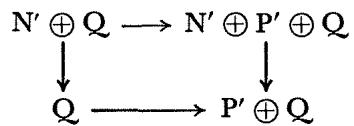
\includegraphics[keepaspectratio]{images/part003_8d12e188.jpg}}

where the horizontal arrows are the canonical injections and the vertical arrows the canonical projections. We derive a commutative diagram

\begin{enumerate}
\def\labelenumi{(\arabic{enumi})}
\setcounter{enumi}{6}
\tightlist
\item
\end{enumerate}

\pandocbounded{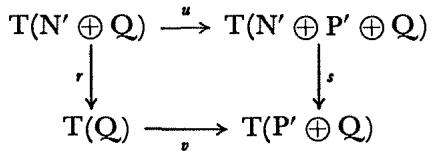
\includegraphics[keepaspectratio]{images/part003_389443db.jpg}}

where r and s are surjective homomorphisms (Proposition 3) and u and v injective homomorphisms. Hence, to prove (6), note that the right hand side is obviously contained in the left; it therefore suffices to verify that if

\[
x \in \mathsf {T} (\mathbf {N} ^ {\prime} \oplus \mathbf {Q}) \cap \mathsf {T} (\mathbf {P} ^ {\prime} \oplus \mathbf {Q}),
\]

then \(x \in \mathsf{T}(\mathsf{Q})\) . Now the definition of the homomorphism s shows that its restriction to \(\mathsf{T}(\mathsf{P}' \oplus \mathsf{Q})\) (identified with a subalgebra of \(\mathsf{T}(\mathsf{N}' \oplus \mathsf{P}' \oplus \mathsf{Q})\)) is the identity mapping; the hypothesis on x therefore implies that \(s(u(x)) = x\) . But then also \(v(r(x)) = x\) , in other words x belongs to the image of \(\mathsf{T}(\mathsf{Q})\) in \(\mathsf{T}(\mathsf{P}' \oplus \mathsf{Q})\) , which was to be proved.

Remark. Note in particular that the hypotheses of Proposition 4 always hold for arbitrary submodules N, P of M when A is a field (II, § 7, no. 3, Proposition 4). Moreover, if N ⊂ P and N ≠ P, then T \(^{n}\) (N) ≠ T \(^{n}\) (P) for all n ≥ 1, since if R is a complement of P in N, then T \(^{n}\) (P) ∩ T \(^{n}\) (R) = \{0\} by (4) and T \(^{n}\) (R) ≠ \{0\}.

COROLLARY. Let K be a commutative field and M a vector space over K. For every element \(z \in \mathsf{T}(\mathbf{M})\) , there exists a smallest vector space N of M such that \(z \in \mathsf{T}(\mathbf{N})\) and N is of finite rank over K.

It is understood in this statement that for every vector subspace P of M, \(T(P)\) is canonically identified with a subalgebra of \(T(M)\) . Let \(z \in T(M)\) ; z can be expressed as a linear combination of elements each of which is a finite product of elements of \(M = T^{1}(M)\) ; all the elements of M which occur in these products generate a vector subspace Q of finite rank and \(z \in T(Q)\) .

Let \(\mathfrak{F}\) be the (non-empty) set of vector subspaces \(\mathbf{P}\) of finite rank such that \(z\in \mathsf{T}(\mathbf{P})\) . Every decreasing sequence of elements of \(\mathfrak{F}\) is stationary, since they are vector spaces of finite rank. Hence \(\mathfrak{F}\) has a minimal element \(\mathbf{N}\) (Set Theory, III, §6, no. 5). It remains to verify that every \(\mathbf{P}\in \mathfrak{F}\) contains \(\mathbf{N}\) ; now, \(z\in \mathsf{T}(\mathbf{P})\cap \mathsf{T}(\mathbf{N}) = \mathsf{T}(\mathbf{P}\cap \mathbf{N})\) (Proposition 4); in view of the definition of \(\mathbf{N}\) , this implies \(\mathbf{N}\cap \mathbf{P} = \mathbf{N}\) , that is \(\mathbf{P}\supset \mathbf{N}\) .

The subspace N of M is said to be associated with z.

\subsection{EXTENSION OF THE RING OF SCALARS}

Let A, A' be two commutative rings and \(\rho:A\to A'\) a ring homomorphism. Let M be an A-module, M' an A'-module and \(u:M\to M'\) an A-homomorphism; as the canonical injection \(\phi_{M'}:M'\to T_{A'}(M')\) is also an A-homomorphism (by restriction of scalars), so is the composition \(M\xrightarrow{u}M'\xrightarrow{\phi_{M'}}T_{A'}(M')\) . An A-algebra homomorphism \(T_{A}(M)\to\rho*(T_{A'}(M'))\) is derived (no. 2), also denoted by \(T(u):T_{A}(M)\to T_{A'}(M')\) , which is the unique A-homomorphism rendering commutative the diagram

\begin{enumerate}
\def\labelenumi{(\arabic{enumi})}
\setcounter{enumi}{7}
\tightlist
\item
\end{enumerate}

\pandocbounded{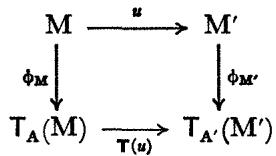
\includegraphics[keepaspectratio]{images/part003_9672ae23.jpg}}

If \(\sigma: \mathbf{A}' \to \mathbf{A}''\) is a commutative ring homomorphism, \(\mathbf{M}''\) an \(\mathbf{A}''\) -module and \(v: \mathbf{M}' \to \mathbf{M}''\) an \(\mathbf{A}'\) -homomorphism, the above uniqueness property shows that

\[
\mathbf {T} (v \circ u) = \mathbf {T} (v) \circ \mathbf {T} (u).\tag{9}
\]

PROPOSITION 5. Let A, B be two commutative rings, \(\rho: \mathbf{A} \to \mathbf{B}\) a ring homomorphism and M an A-module. The canonical extension

\[
\psi : \mathsf {T} _ {\mathbf {B}} (\mathbf {B} \otimes_ {\mathbf {A}} \mathbf {M}) \rightarrow \mathbf {B} \otimes_ {\mathbf {A}} \mathsf {T} _ {\mathbf {A}} (\mathbf {M})
\]

of the B-linear mapping \(\mathbf{1}_{\mathbf{B}} \otimes \phi_{\mathbf{M}}: \mathbf{B} \otimes_{\mathbf{A}} \mathbf{M} \to \mathbf{B} \otimes_{\mathbf{A}} \mathsf{T}_{\mathbf{A}}(\mathbf{M})\) is an isomorphism of graded B-algebras.

Consider the two A-algebra homomorphisms: the canonical injection \(j: \mathbf{B} = \mathsf{T}^0(\mathbf{B} \otimes_{\mathbf{A}} \mathbf{M}) \to \mathsf{T}(\mathbf{B} \otimes_{\mathbf{A}} \mathbf{M})\) and the homomorphism

\[
h = \mathsf {T} (i): \mathsf {T} (\mathbf {M}) \rightarrow \mathsf {T} (\mathbf {B} \otimes_ {\mathbf {A}} \mathbf {M})
\]

derived (cf.~formula (8)) from the canonical A-linear mapping

\[
i: \mathbf {M} \rightarrow \mathbf {B} \otimes_ {\mathbf {A}} \mathbf {M}.
\]

As \(\mathsf{T}^0 (\mathbf{B}\otimes_{\mathbf{A}}\mathbf{M})\) is contained in the centre of \(\mathsf{T}(\mathbf{B}\otimes_{\mathbf{A}}\mathbf{M})\) , Proposition 5 of §4, no. 2 can be applied and an A-algebra homomorphism

\[
\psi^ {\prime}: \mathbf {B} \otimes_ {\mathbf {A}} \mathsf {T} (\mathbf {M}) \rightarrow \mathsf {T} (\mathbf {B} \otimes_ {\mathbf {A}} \mathbf {M})
\]

is obtained such that, for \(\beta \in \mathbf{B}\) , \(x_{i} \in \mathbf{M}\) for \(1 \leqslant i \leqslant n\) ,

\[
\psi^ {\prime} (\beta \otimes (x _ {1} \otimes x _ {2} \otimes \dots \otimes x _ {n})) = \beta ((1 \otimes x _ {1}) \otimes (1 \otimes x _ {2}) \otimes \dots \otimes (1 \otimes x _ {n})),
\]

which shows immediately that \(\psi'\) is also a B-algebra homomorphism. It suffices to prove that \(\psi \circ \psi'\) and \(\psi' \circ \psi\) are the identity mappings on \(B \otimes_{A} T(M)\) and \(T(B \otimes_{A} M)\) respectively. Now, these two algebras are generated by \(B \otimes_{A} M\) and clearly \(\psi \circ \psi'\) and \(\psi' \circ \psi\) coincide with the identity mapping on \(B \otimes_{A} M\) , whence the conclusion.

\subsection{DIRECT LIMIT OF TENSOR ALGEBRAS}

Let \((\mathbf{A}_{\alpha},\phi_{\beta \alpha})\) be a directed direct system of commutative rings and \((\mathbf{M}_{\alpha},f_{\beta \alpha})\) a direct system of \(\mathbf{A}_{\alpha}\) -modules (II, § 6, no. 2); let \(\mathbf{A} = \varinjlim \mathbf{A}_{\alpha}\) and \(\mathbf{M} = \varinjlim \mathbf{M}_{\alpha}\) , which is an A-module. For \(\alpha \leqslant \beta\) an \(\mathbf{A}_{\alpha}\) -algebra homomorphism (no. 3, formula (8)) \(f_{\beta \alpha}' = \mathsf{T}(f_{\beta \alpha})\colon \mathsf{T}_{\mathbf{A}_{\alpha}}(\mathbf{M}_{\alpha})\to \mathsf{T}_{\mathbf{A}_{\beta}}(\mathbf{M}_{\beta})\) is derived canonically from the \(\mathbf{A}_{\alpha}\) -homomorphism \(f_{\beta \alpha}\colon \mathbf{M}_{\alpha}\to \mathbf{M}_{\beta}\) and it follows from (9) (no. 3) that \((\mathsf{T}_{\mathbf{A}_{\alpha}}(\mathbf{M}_{\alpha}),f_{\beta \alpha}')\) is a direct system of \(\mathbf{A}_{\alpha}\) -algebras. On the other hand let \(f_{\alpha}\colon \mathbf{M}_{\alpha}\to \mathbf{M}\) be the canonical \(\mathbf{A}_{\alpha}\) -homomorphism; an \(\mathbf{A}_{\alpha}\) -algebra homomorphism \(f_{\alpha}'\colon \mathsf{T}_{\mathbf{A}_{\alpha}}(\mathbf{M}_{\alpha})\to \mathsf{T}_{\mathbf{A}}(\mathbf{M})\) is derived (no. 3, formula (8)) and it also follows from (9) (no. 3) that the \(f_{\alpha}'\) constitute a direct system of \(\mathbf{A}_{\alpha}\) -homomorphisms.

PROPOSITION 6. The A-homomorphism \(f' = \varinjlim f_{\alpha}' : \varinjlim T_{A_{\alpha}}(M_{\alpha}) \to T_{A}(M)\) is a graded algebra isomorphism.

To simplify we write \(\mathbf{E} = T_{\mathbf{A}}(\mathbf{M})\) and \(\mathbf{E}' = \varinjlim T_{\mathbf{A}_{\alpha}}(\mathbf{M}_{\alpha})\) and let

\[
g _ {\alpha}: \mathsf {T} _ {\mathrm{A} _ {\alpha}} (\mathbf {M} _ {\alpha}) \rightarrow \mathbf {E} ^ {\prime}
\]

be the canonical \(\mathbf{A}_{\alpha}\) -homomorphism. Clearly the composite \(\mathbf{A}_{\alpha}\) -linear mappings \(\mathbf{M}_{\alpha} \xrightarrow{\phi_{\mathbf{M}_{\alpha}}} \mathsf{T}_{\mathbf{A}_{\alpha}}(\mathbf{M}_{\alpha}) \xrightarrow{g_{\alpha}} \mathbf{E}'\) form a direct system and there is therefore one and only one A-linear mapping \(u = \varinjlim (g_{\alpha} \circ \phi_{\mathbf{M}_{\alpha}}): \mathbf{M} \to \mathbf{E}'\) such that

\[
u \circ f _ {\alpha} = g _ {\alpha} \circ \phi_ {M _ {\alpha}}
\]

for all \(\alpha\) . This mapping itself factorizes uniquely (no. 1, Proposition 1) into \(\mathbf{M} \xrightarrow{\phi_{\mathbf{M}}} \mathrm{E} \to \mathrm{E}'\) , where \(h\) is an A-algebra homomorphism. It will suffice to prove that \(h \circ f' = 1_{\mathrm{E}'}\) and \(f' \circ h = 1_{\mathrm{E}}\) .

To this end note that, for every index \(\alpha\) , (no. 3, formula (8))

\[
h \circ f _ {\alpha} ^ {\prime} \circ \phi_ {M _ {\alpha}} = h \circ \phi_ {M} \circ f _ {\alpha} = u \circ f _ {\alpha} = g _ {\alpha} \circ \phi_ {M _ {\alpha}}
\]

whence, by the uniqueness assertion of no. 1, Proposition 1,

\[
h \circ f _ {\alpha} ^ {\prime} = g _ {\alpha}
\]

for all \(\alpha\) ; it follows that \((h \circ f') \circ g_{\alpha} = g_{\alpha}\) for all \(\alpha\) and hence \(h \circ f' = 1_{\mathbf{E}'}\) by definition of a direct limit.

On the other hand, by virtue of no. 3, formula (8),

\[
f ^ {\prime} \circ u \circ f _ {\alpha} = f ^ {\prime} \circ g _ {\alpha} \circ \phi_ {M _ {\alpha}} = f _ {\alpha} ^ {\prime} \circ \phi_ {M _ {\alpha}} = \phi_ {M} \circ f _ {\alpha},
\]

whence again \(f' \circ u = \phi_{\mathbb{M}}\) by definition of a direct limit; we conclude that \(f' \circ h \circ \phi_{\mathbb{M}} = \phi_{\mathbb{M}}\) and the uniqueness property of no. 1, Proposition 1 gives \(f' \circ h = 1_{\mathbb{E}}\) .

Proposition 6 can also be shown by observing that, for every integer \(n \geqslant 1\) , there is a canonical A-module isomorphism \(\lim_{\longrightarrow} \mathsf{T}_{\mathbf{A}_{\alpha}}^{n}(\mathbf{M}_{\alpha}) \to \mathsf{T}_{\mathbf{A}}^{n}(\mathbf{M})\) , as follows by induction on \(n\) from II, § 6, no. 3, Proposition 7. It is immediately verified that these isomorphisms are the restrictions of \(f'\) .

\subsection{TENSOR ALGEBRA OF A DIRECT SUM. TENSOR ALGEBRA OF A FREE MODULE. TENSOR ALGEBRA OF A GRADED MODULE}

Let A be a commutative ring and \(M = \bigoplus_{\lambda \in L} M_{\lambda}\) the direct sum of a family of A-modules. It follows from II, §3, no. 7, Proposition 7, by induction on n, that \(T^{n}(M)\) is the direct sum of the submodules the images of the canonical injections

\[
\mathbf {M} _ {\lambda_ {1}} \otimes \mathbf {M} _ {\lambda_ {2}} \otimes \dots \otimes \mathbf {M} _ {\lambda_ {n}} \rightarrow \mathsf {T} ^ {n} (\mathbf {M}) = \mathbf {M} ^ {\otimes n}
\]

relative to all the sequences \((\lambda_{i})\in\mathbf{L}^{n}\) . Identifying \(M_{\lambda_{1}}\otimes M_{\lambda_{2}}\otimes\cdots\otimes M_{\lambda_{n}}\) with this image, it is seen that \(T(\mathbf{M})\) is the direct sum of all the modules

\[
\mathbf {M} _ {\lambda_ {1}} \otimes \mathbf {M} _ {\lambda_ {2}} \otimes \dots \otimes \mathbf {M} _ {\lambda_ {n}}
\]

where \(n\) runs through \(\mathbf{N}\) and, for each \(n\) , \((\lambda_t)\) runs through \(\mathbf{L}^n\) .

We first deduce the following consequence:

THEOREM 1. Let A be a commutative ring, M a free A-module and \((e_{\lambda})_{\lambda \in L}\) a basis of M. Then the elements \(e_{s} = e_{\lambda_{1}} \otimes e_{\lambda_{2}} \otimes \cdots \otimes e_{\lambda_{n}}\) , where \(s = (\lambda_{1}, \ldots, \lambda_{n})\) runs through the set of all finite sequences of elements of L and \(e_{\varnothing}\) is used to denote the unit element of T(M), form a basis of the A-module T(M).

The elements of this basis are obviously homogeneous and the multiplication table is given by

\[
e _ {s} e _ {t} = e _ {s t}\tag{10}
\]

where \(st\) denotes the sequence of elements of \(\mathbf{L}\) obtained by juxtaposing the sequences \(s\) and \(t\) (I, § 7, no. 2).

It is seen that the basis \((e_{s})\) of T(M), with the multiplicative law (10), is canonically isomorphic to the free monoid of the set L (I, §7, no. 2), the isomorphism being obtained by mapping each word s of this monoid to the element \(e_{s}\) . It follows (§2, no. 7) that the tensor algebra T(M) of a free module M, with a basis of indexing set L, is canonically isomorphic to the free associative algebra of L over A. In particular (§2, no. 7, Proposition 7), for every mapping \(f: L \to E\) from L to an A-algebra E, there exists one and only one A-algebra homomorphism \(\bar{f}: T(M) \to E\) such that \(\bar{f}(e_{\lambda}) = f(\lambda)\) .

Remark. The above results can equally be obtained as a consequence of the universal properties of the free associative algebra and of the tensor algebra, using II, § 3, no. 7, Corollary 2 to Proposition 7.

COROLLARY. If M is a projective A-module, T(M) is a projective A-module.

M is a direct factor of a free A-module N (II, §2, no. 2, Proposition 4) and hence T(M) is a direct factor of T(N) (no. 2); as T(N) is free (Theorem 1), this shows that T(M) is projective (II, §2, no. 2).

PROPOSITION 7. Let \(\Delta\) be a commutative monoid, \(\mathbf{M}\) a graded A-module of type \(\Delta\) and \((\mathbf{M}_{\alpha})_{\alpha \in \Delta}\) its graduation. For every ordered pair \((\alpha, n) \in \Delta \times \mathbf{N}\) , let \(\mathsf{T}^{\alpha,n}(\mathbf{M})\) be the (direct) sum of the submodules \(\mathbf{M}_{\alpha_1} \otimes \mathbf{M}_{\alpha_2} \otimes \dots \otimes \mathbf{M}_{\alpha_n}\) of \(\mathsf{T}^n(\mathbf{M})\) such that \(\sum_{i=1}^{n} \alpha_i = \alpha\) ; then \((T^{\alpha, n}(M))_{(\alpha, n) \in \Delta \times N}\) is the only graduation of type \(\Delta \times N\) compatible with the algebra structure on \(T(M)\) and inducing on \(M = T^1(M)\) the given graduation.

It has been seen at the beginning of this no. that \(\mathsf{T}(\mathbf{M})\) is the direct sum of the \(\mathsf{T}^{\alpha,n}(\mathbf{M})\) and the fact that this is a graduation compatible with the algebra structure follows immediately from the definitions. If \((\mathsf{T}'^{\alpha,n})\) is another graduation of type \(\Delta \times \mathbf{N}\) on \(\mathsf{T}(\mathbf{M})\) compatible with the algebra structure and such that \(\mathsf{T}^{\alpha,1}(\mathbf{M}) = \mathsf{T}'^{\alpha,1}\) for \(\alpha \in \Delta\) , it follows immediately from the definitions that, for all \(n \geqslant 1\) and all \(\alpha \in \Delta\) , \(\mathsf{T}^{\alpha,n}(\mathbf{M}) \subset \mathsf{T}'^{\alpha,n}\) ; but since \(\mathsf{T}(\mathbf{M})\) is also the direct sum of the \(\mathsf{T}^{\alpha,n}(\mathbf{M})\) , this implies that \(\mathsf{T}'^{\alpha,n} = \mathsf{T}^{\alpha,n}(\mathbf{M})\) (II, § 1, no. 8, Remark).

\subsection{TENSORS AND TENSOR NOTATION}

Let A be a commutative ring, M an A-module, \(\mathbf{M}^*\) the dual of M (II, § 2, no. 3) and I and J two disjoint finite sets; the A-module \(\bigotimes_{i\in \mathrm{I}\cup \mathrm{J}}\mathbf{E}_i\) , where \(\mathbf{E}_i = \mathbf{M}\) if \(i\in \mathrm{I}\) , \(\mathbf{E}_i = \mathbf{M}^*\) if \(i\in \mathrm{J}\) , is denoted by \(\mathsf{T}_{\mathsf{J}}^{\mathsf{I}}(\mathbf{M})\) ; the elements of \(\mathsf{T}_{\mathsf{J}}^{\mathsf{I}}(\mathbf{M})\) are called tensors of type (I,J) over M. They are called contravariant if \(\mathbf{J} = \varnothing\) , covariant if \(\mathbf{I} = \varnothing\) and mixed otherwise.

Let \(I'\) , \(I''\) be two subsets of I and \(J'\) , \(J''\) two subsets of J such that \(I' \cup I'' = I\) , \(\mathbf{I}' \cap \mathbf{I}'' = \varnothing, \mathbf{J}' \cup \mathbf{J}'' = \mathbf{J}, \mathbf{J}' \cap \mathbf{J}'' = \varnothing\) ; then there is a canonical associativity isomorphism (II, § 3, no. 9)

\[
\mathsf {T} _ {\mathbf {J}} ^ {\mathbf {I}} (\mathbf {M}) \rightarrow \mathsf {T} _ {\mathbf {J} ^ {\prime}} ^ {\mathbf {I} ^ {\prime}} (\mathbf {M}) \otimes_ {\mathbf {A}} \mathsf {T} _ {\mathbf {J} ^ {\prime \prime}} ^ {\mathbf {I} ^ {\prime \prime}} (\mathbf {M}).\tag{11}
\]

Considering the tensor algebra \(\mathsf{T}(\mathbf{M}\oplus \mathbf{M}^{*})\) , it follows from no. 5 that \(\mathsf{T}^n (\mathbf{M}\oplus \mathbf{M}^*)\) is canonically identified with the direct sum of the \(\mathsf{T}_{\mathbf{J}}^{\mathbf{I}}(\mathbf{M})\) where I runs through the set of subsets of the interval \([1,n]\) of \(\mathbf{N}\) and J is the complement of I in \([1,n]\) .

When \(I = [1, p]\) and \(J = [p + 1, p + q]\) with integers \(p \geqslant 0\) , \(q \geqslant 0\) (where we replace I (resp. J) by \(\varnothing\) when \(p = 0\) (resp. \(q = 0\) )), the A-module \(T_J^I(M)\) is also denoted by \(T_q^p(M)\) ; the A-modules \(T_0^n(M)\) and \(T_n^0(M)\) are therefore by definition the A-modules \(T^n(M)\) and \(T^n(M^*)\) respectively. When I and J are arbitrary finite sets of cardinals \(p = \text{Card}(I)\) and \(q = \text{Card}(J)\) , we give each of them a total ordering; then there exists an increasing bijection of I (resp. J) onto \([1, p]\) (resp. \([p + 1, p + q]\) ) and these bijections therefore define an isomorphism

\[
\mathbf {T} _ {\mathrm{J}} ^ {\mathrm{I}} (\mathbf {M}) \rightarrow \mathbf {T} _ {q} ^ {p} (\mathbf {M}).
\]

When M is a finitely generated projective A-module, it follows from II, § 2, no. 7, Corollary 4 to Proposition 13 and II, § 4, no. 4, Corollary 1 to Proposition 4 that there is a canonical isomorphism

\[
(\mathsf {T} _ {\mathbf {J}} ^ {\mathbf {I}} (\mathbf {M})) ^ {*} \to \mathsf {T} _ {\mathbf {I}} ^ {\mathbf {J}} (\mathbf {M}).
\]

Suppose now that \(\mathbf{M}\) is a finitely generated free A-module and let \((e_{\lambda})_{\lambda \in L}\) be a basis of \(\mathbf{M}\) (L therefore being a finite set). The basis of \(\mathbf{M}^*\) dual to \((e_{\lambda})\) (II, §2, no. 6) is denoted by \((e^{\lambda})_{\lambda \in L}\) . The bases \((e_{\lambda})\) and \((e^{\lambda})\) of \(\mathbf{M}\) and \(\mathbf{M}^*\) respectively define (no. 5) a basis of \(\mathsf{T}_{\mathbf{J}}^{\mathbf{I}}(\mathbf{M})\) , which we give explicitly as follows: given two mappings \(f\colon \mathbf{I} \to \mathbf{L}\) and \(g\colon \mathbf{J} \to \mathbf{L}\) , let \(e_f^g\) be the element \(\bigotimes_{i \in I \cup J} x_i\) of \(\mathsf{T}_{\mathbf{J}}^{\mathbf{I}}(\mathbf{M})\) defined by

\[
x _ {i} = e _ {f (i)} \quad \text { if } i \in \mathbf {I}, \qquad x _ {i} = e ^ {g (i)} \quad \text { if } i \in \mathbf {J}.
\]

When \((f, g)\) runs through the set of ordered pairs of mappings \(f: \mathbf{I} \to \mathbf{L}\) and \(g: \mathbf{J} \to \mathbf{L}\) , the \(e_f^g\) form a basis of the A-module \(\mathsf{T}_{\mathbf{J}}^{\mathbf{I}}(\mathbf{M})\) , said to be associated with the given basis \((e_{\lambda})\) of \(\mathbf{M}\) . For \(z \in \mathsf{T}_{\mathbf{J}}^{\mathbf{I}}(\mathbf{M})\) , we can therefore write

\[
z = \sum_ {(f, g)} \alpha_ {g} ^ {f} (z). e _ {f} ^ {g}\tag{12}
\]

where the \(\alpha_g^f\) are the coordinate forms relative to the basis \((e_f^g)\) ; by an abuse of language, the \(\alpha_g^f(z)\) are called the coordinates of the tensor \(z\) with respect to the basis \((e_\lambda)\) of the module M. The \(\alpha_g^f\) constitute the dual basis of \((e_g^f)\) , in other words they are identified with the elements of the basis of \(\mathsf{T}_{\mathbf{I}}^{\mathbf{j}}(\mathbf{M})\) , associated with \((e_\lambda)\) . When I and J are complementary subsets of an interval \([1,n]\) of N, \(\alpha_g^f\) (or \(\alpha_g^f(z)\) ) is denoted as follows: each element \(f(i)\) for \(i\in I\) is written as an upper index in the \(i\) -th place with a dot in the \(i\) -th place for \(i \in \mathbf{J}\) ; similarly, \(g(i)\) for \(i \in \mathbf{J}\) is written as a lower index in the \(i\) -th place with a dot in the \(i\) -th place for \(i \in \mathbf{I}\) . For example, for \(\mathbf{I} = \{1, 4\}\) , \(\mathbf{J} = \{2, 3\}\) , we write \(\alpha_{\cdot \nu \rho}^{\lambda \cdot \cdot \mu}\) if \(f(1) = \lambda, f(4) = \mu, g(2) = \nu, g(3) = \rho\) .

Let \((\bar{e}_{\lambda})_{\lambda \in L}\) be another basis of M and \(P\) the matrix of passing from \((e_{\lambda})\) to \((\bar{e}_{\lambda})\) (II, § 10, no. 8). Then the matrix of passing from \((e^{\lambda})\) to \((\bar{e}^{\lambda})\) (dual basis of \((\bar{e}_{\lambda}))\) is the contragredient \(^{t}P^{-1}\) of \(P\) (II, § 10, no. 8, Proposition 5). It follows (II, § 10, no. 10) that the matrix of passing from the basis \((e_{f}^{g})\) of \(\mathrm{T}_{\mathrm{J}}^{\mathrm{I}}(\mathrm{M})\) to the basis \((\bar{e}_{f}^{g})\) (where \(f\) (resp. \(g\) ) runs through the set of mappings of I into L (resp. of J into L)) is the matrix

\[
\bigotimes_ {i \in I \cup J} Q _ {i}, \quad \text { where } Q _ {i} = P \text { if } i \in I, Q _ {i} = ^ {t} P ^ {- 1} \text { if } i \in J.\tag{13}
\]

The transpose of this matrix is therefore identified with

\[
\bigotimes_ {i \in \mathbf {I} \cup J} R _ {i}, \quad \text { where } R _ {i} = ^ {t} P ^ {- 1} \text { if } i \in \mathbf {I}, R _ {i} = P \text { if } i \in \mathbf {J}.\tag{14}
\]

Suppose now that \(\mathbf{M}\) is an arbitrary module. Let \(i\in \mathbf{I}, j\in \mathbf{J}\) and write \(\mathbf{I}' = \mathbf{I} - \{i\}, J' = J - \{j\}\) ; we shall define a canonical A-linear mapping

\[
c _ {j} ^ {i} \colon \mathsf {T} _ {\mathbf {J}} ^ {\mathbf {I}} (\mathbf {M}) \to \mathsf {T} _ {\mathbf {J} ^ {\prime}} ^ {\mathbf {I} ^ {\prime}} (\mathbf {M}),
\]

called contraction of the index \(i\) and the index \(j\) . For this, note that the mapping of \(\mathbf{M}^{\mathrm{I}} \times (\mathbf{M}^{*})^{\mathrm{J}}\) , which associates with every family \((x_{i})_{i \in \mathbf{I} \cup \mathbf{J}}\) , where \(x_{i} \in \mathbf{M}\) if \(i \in \mathbf{I}\) and \(x_{i} \in \mathbf{M}^{*}\) if \(i \in \mathbf{J}\) , the element

\[
\left\langle x _ {i}, x _ {j} \right\rangle \otimes_ {k \in (\mathbb {I} \cup \mathbb {J}) - \{i, j \}} x _ {k}\tag{15}
\]

of \(T_{J'}^{I'}(M)\) , is A-multilinear; \(c_{j}^{i}\) is the corresponding A-linear mapping.

Suppose now that M is free and finitely generated and let \((e_{\lambda})_{\lambda \in L}\) be a basis of M. Given two mappings \(f: I \to L\) , \(g: J \to L\) , let \(f_i\) denote the restriction of f to \(I' = I - \{i\}\) and \(g_j\) the restriction of g to \(J' = J - \{j\}\) ; then by virtue of (12)

\[
c _ {j} ^ {i} (e _ {f} ^ {g}) = \left\{ \begin{array}{l l} 0 & \text { if } f (i) \neq g (j) \\ e _ {f _ {i}} ^ {g _ {j}} & \text { if } f (i) = g (j) \end{array} \right.\tag{16}
\]

The expression for the coordinates of \(c_j^i(z)\) as a function of those of \(z\) is obtained; for every mapping \(f'\) (resp. \(g'\) ) of \(I'\) into \(L\) (resp. of \(J'\) into \(L\) ) and every \(\lambda \in L\) , let \((f', \lambda)\) (resp. \((g', \lambda)\) ) denote the mapping of \(I\) into \(L\) (resp. of \(J\) into \(L\) ) whose restriction to \(I'\) (resp. \(J'\) ) is \(f'\) (resp. \(g'\) ) and which takes the value \(\lambda\) at the element \(i\) (resp. \(j\) ). Then, if the coordinate forms relative to the basis \((e_{f'}^{g'})\) of \(T_{J'}^{I'}(M)\) are denoted by \(\beta_{g'}^{f'}\) ,

\[
\beta_ {g ^ {\prime}} ^ {f ^ {\prime}} (c _ {j} ^ {i} (z)) = \sum_ {\lambda \in L} \alpha_ {(g ^ {\prime}, \lambda)} ^ {(f ^ {\prime}, \lambda)} (z).\tag{17}
\]

Examples of tensors. (1) Let M be a finitely generated projective A-module. We know (II, § 4, no. 2, Corollary to Proposition 2), that there is a canonical A-module isomorphism

\[
\theta_ {\mathbf {M}} \colon \mathbf {M} ^ {*} \otimes_ {\mathbf {A}} \mathbf {M} \rightarrow \operatorname{End} _ {\mathbf {A}} (\mathbf {M})
\]

such that \(\theta_{\mathbf{M}}(x^{*}\otimes x)\) (for \(x\in \mathbf{M},x^{*}\in \mathbf{M}^{*}\) ) is the endomorphism

\[
y \mapsto \langle y, x ^ {*} \rangle x.
\]

Hence, by means of \(\theta_{\mathbf{M}}\) , \(\mathsf{T}_{(1)}^{(2)}(\mathbf{M})\) (isomorphic to \(\mathsf{T}_1^1 (\mathbf{M}))\) can be identified with the A-module \(\operatorname{End}_{\mathbf{A}}(\mathbf{M})\) . Suppose that \(\mathbf{M}\) is a free module and let \((e_{\lambda})_{\lambda \in \mathbf{L}}\) be a basis of \(\mathbf{M}\) ; then the coordinates of a tensor \(z\in \mathbf{M}^*\otimes \mathbf{M}\) relative to the basis \((e^{\mu}\otimes e_{\lambda})\) of this module are denoted by \(\zeta_{\mu}^{\cdot \lambda}\) . As \(\theta_{\mathrm{M}}(e^{\mu}\otimes e_{\lambda})\) is the endomorphism \(y\mapsto \langle y,e^{\mu}\rangle e_{\lambda}\) , the endomorphism \(u = \theta_{\mathrm{M}}(z) = \theta_{\mathrm{M}}\left(\sum_{\lambda ,\mu}\zeta_{\mu}^{\cdot \lambda}e^{\mu}\otimes e_{\lambda}\right)\) maps \(y\) to \(\sum_{\lambda ,\mu}\zeta_{\mu}^{\cdot \lambda}\langle y,e^{\mu}\rangle e_{\lambda}\) ; writing \(y = e_{\lambda}\) , we obtain the relation

\[
u (e _ {\lambda}) = \sum_ {\mu \in L} \zeta_ {\lambda} ^ {\cdot \mu} e _ {\mu}\tag{18}
\]

in other words, the matrix of the linear mapping \(u = \theta_{\mathrm{M}}(z)\) is that whose element in the row of index \(\mu\) and column of index \(\lambda\) is \(\zeta_{\lambda}^{\mu}\) .

The definition of the trace of \(u\) (II, § 4, no. 3) shows immediately that

\[
\operatorname{Tr} (\theta_ {\mathbb {M}} (z)) = c _ {1} ^ {2} (z).
\]

Therefore the element \(z_0 = \sum_{\lambda \in L} e^\lambda \otimes e_\lambda\) (whose coordinates \(\zeta_\mu^{\cdot \lambda}\) are zero for \(\lambda \neq \mu\) and equal to 1 for \(\lambda = \mu\) ), which is such that \(\theta_M(z_0) = 1_M\) , is the image of the element \(1 \in A = T_0^0(M)\) under the mapping the transpose of the contraction

\[
c _ {1} ^ {2}: \mathbf {T} _ {\{1 \}} ^ {\{2 \}} (\mathbf {M}) \rightarrow \mathbf {A}.
\]

\begin{enumerate}
\def\labelenumi{(\arabic{enumi})}
\setcounter{enumi}{1}
\tightlist
\item
  Suppose always that M is a finitely generated projective A-module; there is a canonical A-module isomorphism
\end{enumerate}

\[
\mu : \mathbf {M} ^ {*} \otimes_ {\mathbf {A}} \mathbf {M} ^ {*} \rightarrow (\mathbf {M} \otimes_ {\mathbf {A}} \mathbf {M}) ^ {*}
\]

(II, § 4, no. 4, Corollary 1 to Proposition 2) and a canonical isomorphism

\[
\theta : (\mathbf {M} \otimes_ {\mathbf {A}} \mathbf {M}) ^ {*} \otimes_ {\mathbf {A}} \mathbf {M} \rightarrow \operatorname{Hom} _ {\mathbf {A}} (\mathbf {M} \otimes_ {\mathbf {A}} \mathbf {M}, \mathbf {M})
\]

(II, §4, no. 2, Corollary to Proposition 2); also \(\operatorname{Hom}_{\mathbf{A}}(\mathbf{M} \otimes_{\mathbf{A}} \mathbf{M}, \mathbf{M})\) is canonically isomorphic to the A-module \(\mathcal{L}_2(\mathbf{M}, \mathbf{M}; \mathbf{M})\) of A-bilinear mappings of \(\mathbf{M} \times \mathbf{M}\) into \(\mathbf{M}\) (II, §3, no. 9). Composing these isomorphisms, a canonical isomorphism is obtained

\[
\chi_ {\mathbf {M}} \colon T _ {\{1, 2 \}} ^ {(3)} (\mathbf {M}) = \mathbf {M} ^ {*} \otimes \mathbf {M} ^ {*} \otimes \mathbf {M} \rightarrow \mathcal {L} _ {2} (\mathbf {M}, \mathbf {M}; \mathbf {M})
\]

such that, for \(x^{*}, y^{*}\) in \(\mathbf{M}^{*}\) , \(z \in \mathbf{M}\) , \(\chi_{\mathbf{M}}(x^{*} \otimes y^{*} \otimes z)\) is the bilinear mapping

\[
(u, v) \mapsto \langle u, x ^ {*} \rangle \langle v, y ^ {*} \rangle z.
\]

Hence, by means of \(\chi_{\mathbf{M}}\) , \(\mathsf{T}_{\{1,2\}}^{(3)}(\mathbf{M})\) (isomorphic to \(\mathsf{T}_{2}^{1}(\mathbf{M})\) ) can be identified with the A-module \(\mathcal{L}_2(\mathbf{M},\mathbf{M};\mathbf{M})\) . Suppose that \(\mathbf{M}\) is a free A-module and let \((e_{\lambda})_{\lambda \in L}\) be a basis of \(\mathbf{M}\) ; then the coordinates of a tensor \(z\in \mathbf{M}^*\otimes \mathbf{M}^*\otimes \mathbf{M}\) relative to the basis \((e^{\lambda}\otimes e^{\mu}\otimes e_{\nu})\) of this module are denoted by \(\zeta_{\lambda \mu}^{\cdot \cdot \nu}\) . The bilinear mapping \(\chi_{\mathbf{M}}(z)\) maps the ordered pair \((e_{\lambda},e_{\mu})\) to

\[
\sum_ {\nu \in L} \zeta_ {\lambda \mu}^{\cdot \cdot \nu} e _ {\nu}
\]

and therefore the \(\zeta_{\lambda \mu}^{\cdots \nu}\) are just the constants of structure of the (in general non-associative) algebra defined on \(\mathbf{M}\) by the bilinear mapping \(\chi_{\mathbf{M}}(z)\) , with respect to the basis \((e_{\lambda})\) ( \(\S 1\) , no. 7).

Remark 2. Let \((e_{\lambda})_{\lambda \in L}, (\tilde{e}_{\lambda})_{\lambda \in L}\) be two bases of M and \(P\) the matrix of passage from \((e_{\lambda})\) to \((\tilde{e}_{\lambda})\) . On account of what was seen in Example 1, the element of \(P\) appearing in the row of index \(\lambda\) and the column of index \(\mu\) is denoted by \(\alpha_{\mu}^{\lambda}\) and the element of the contragredient \(^{t}P^{-1}\) appearing in the row of index \(\lambda\) and the column of index \(\mu\) is denoted by \(\beta_{\lambda}^{\mu}\) . Then (in the notation introduced above)

\begin{enumerate}
\def\labelenumi{(\arabic{enumi})}
\setcounter{enumi}{18}
\tightlist
\item
\end{enumerate}

\[
\left\{ \begin{array}{l} \tilde {e} _ {\mu} = \sum_ {\lambda} \alpha_ {\mu} ^ {\lambda} e _ {\lambda} \\ \tilde {e} ^ {\mu} = \sum_ {\lambda} \beta_ {\lambda} ^ {\mu} e ^ {\lambda} \end{array} \right.\tag{20}
\]

\[
\bar {e} _ {f ^ {\prime}} ^ {g ^ {\prime}} = \sum_ {(f, g)} \left(\prod_ {i \in I} \alpha_ {f ^ {\prime} (i)} ^ {f (i)}\right) \left(\prod_ {j \in J} \beta_ {g (j)} ^ {g ^ {\prime} (j)}\right) e _ {f} ^ {g}
\]

for all mappings \(f': \mathbf{I} \to \mathbf{L}\) and \(g': \mathbf{J} \to \mathbf{L}\) . The coordinates \(\zeta_g^f\) of a tensor \(z \in \mathbb{T}_J^{\mathbf{I}}(\mathbf{M})\) with respect to the basis \((e_{\lambda})\) can therefore be expressed in terms of the coordinates \(\bar{\zeta}_{g'}^{f'}\) of \(z\) with respect to the basis \((\bar{e}_{\lambda})\) using the formulae

\[
\zeta_ {g} ^ {f} = \sum_ {(f ^ {\prime}, g ^ {\prime})} \left(\prod_ {i \in I} \alpha_ {f ^ {\prime} (i)} ^ {f (i)}\right) \left(\prod_ {j \in J} \beta_ {g (j)} ^ {g ^ {\prime} (j)}\right) \bar {\zeta} _ {g ^ {\prime}} ^ {f ^ {\prime}}.\tag{21}
\]

The matrix \(P^{-1}\) of passage from the basis \((\tilde{e}_{\lambda})\) to the basis \((e_{\lambda})\) is the transpose of \(^{t}P^{-1}\) , so that \(\beta_{\lambda}^{\mu}\) is the element which appears in the column of index \(\lambda\) and the row of index \(\mu\) of \(P^{-1}\) . The calculation of \(e_{f}^{g}\) in terms of the \(\tilde{e}_{f'}^{g'}\) and that of the \(\overline{\zeta}_{g'}^{f'}\) in terms of the \(\zeta_{g}^{f}\) are therefore made by replacing \(\alpha_{\mu}^{\lambda}\) by \(\beta_{\lambda}^{\mu}\) and \(\beta_{\lambda}^{\mu}\) by \(\alpha_{\mu}^{\lambda}\) in the above calculations and exchanging the roles of \(f\) and \(f'\) and those of \(g\) and \(g'\) . Then

\[
e _ {f} ^ {g} = \sum_ {(f ^ {\prime}, g ^ {\prime})} \left(\prod_ {j \in J} \alpha_ {g ^ {\prime} (j)} ^ {g (j)}\right) \left(\prod_ {i \in I} \beta_ {f (i)} ^ {f ^ {\prime} (i)}\right) \bar {e} _ {f ^ {\prime}} ^ {g ^ {\prime}}\tag{22}
\]

\[
\bar {\zeta} _ {g ^ {\prime}} ^ {f ^ {\prime}} = \sum_ {(f, g)} \left(\prod_ {j \in J} \alpha_ {g ^ {\prime} (j)} ^ {g (j)}\right) \left(\prod_ {i \in I} \beta_ {f (i)} ^ {f ^ {\prime} (i)}\right) \zeta_ {g} ^ {f}.\tag{23}
\]

The above formulae are such that the summation is over indices which appear once as a lower index and once as an upper index. Certain authors allow themselves because of this circumstance to suppress the summation signs.

\section{SYMMETRIC ALGEBRAS}

\subsection{DEFINITION OF THE SYMMETRIC ALGEBRA OF A MODULE}

DEFINITION 1. Let A be a commutative ring and M an A-module. The symmetric algebra of M, denoted by S(M), or Sym(M), or \(S_{A}(M)\), is the quotient algebra over A of the tensor algebra T(M) by the two-sided ideal \(\mathfrak{J}'\) (also denoted by \(\mathfrak{J}_{\mathbf{M}}'\) ) generated by the elements \(xy - yx = x \otimes y - y \otimes x\) of T(M), where \(x\) and \(y\) run through M.

Since the ideal \(\mathfrak{J}'\) is generated by homogeneous elements of degree 2, it is a graded ideal (II, §11, no. 3, Proposition 2); we write \(\mathfrak{J}_n' = \mathfrak{J}' \cap T^n(M)\) ; the algebra \(S(M)\) is then graded by the graduation (called canonical) consisting of the \(S^n(M) = T^n(M)/\mathfrak{J}_n'\) . Now \(\mathfrak{J}_0' = \mathfrak{J}_1' = \{0\}\) and hence \(S^0(M)\) is canonically identified with A and \(S^1(M)\) with \(T^1(M) = M\) ; we shall always make these identifications in what follows and denote by \(\phi'\) or \(\phi_M'\) the canonical injection \(M \to S(M)\) .

PROPOSITION 1. The algebra \(\mathbf{S}(\mathbf{M})\) is commutative.

By definition \(\phi'(x)\phi'(y) = \phi'(y)\phi'(x)\) for \(x, y\) in \(\mathbf{M}\) and, as the elements \(\phi'(x)\) , where \(x\) runs through \(\mathbf{M}\) , generate \(\mathbf{S}(\mathbf{M})\) , the conclusion follows from §1, no. 7.

PROPOSITION 2. Let E be an A-algebra and f: M → E an A-linear mapping such that

\[
f (x) f (y) = f (y) f (x) \text {   for   all   } x, y \text {   in   } \mathbf {M}.\tag{1}
\]

There exists one and only one A-algebra homomorphism \(g \colon \mathbb{S}(\mathbf{M}) \to \mathbf{E}\) such that \(f = g \circ \phi'\) .

In other words, \((\mathbb{S}(\mathbf{M}), \phi')\) is a solution of the universal mapping problem (Set Theory, IV, §3, no. 1), where \(\Sigma\) is the species of A-algebra structure, the \(\alpha\) -mappings being the linear mappings of the A-module M to an A-algebra satisfying (1).

The uniqueness of \(g\) follows from the fact that \(\phi'(\mathbf{M}) = \mathbf{M}\) generates \(\mathbf{S}(\mathbf{M})\) . To prove the existence of \(g\) , note that by virtue of § 5, no.~1, Proposition 1 there exists an A-algebra homomorphism \(g_1: \mathbf{T}(\mathbf{M}) \to \mathbf{E}\) such that \(f = g_1 \circ \phi\) ;

all that needs to be proved is that \(g_1\) is zero on the ideal \(\mathfrak{J}'\) , for then, if \(p: \mathsf{T}(\mathbf{M}) \to \mathsf{S}(\mathbf{M}) = \mathsf{T}(\mathbf{M}) / \mathfrak{J}'\) is the canonical homomorphism, we can write \(g_1 = g \circ p\) , where \(g: \mathsf{S}(\mathbf{M}) \to \mathbf{E}\) is an algebra homomorphism, and the conclusion will follow from the fact that \(p \circ \phi = \phi'\) . Now the kernel of \(g_1\) is a two-sided ideal which, by virtue of (1) and the relation \(g_1 \circ \phi = f\) , contains the elements \(x \otimes y - y \otimes x\) for \(x, y\) in \(\mathbf{M}\) . This completes the proof.

Remarks. (1) Suppose that E is a graded A-algebra of type Z, with graduation \((\mathrm{E}_{n})\) , and suppose also that the linear mapping f (assumed to satisfy (1)) is such that

\[
f (\mathbf {M}) \subset \mathrm{E} _ {1}.\tag{2}
\]

Then the relation \(g(x_1x_2 \ldots x_p) = f(x_1)f(x_2) \ldots f(x_p)\) with the \(x_i \in \mathbf{M}\) shows that \(g(\mathbf{S}^p(\mathbf{M})) \subset \mathrm{E}_p\) for all \(p \geqslant 0\) and hence \(g\) is a graded algebra homomorphism.

\begin{enumerate}
\def\labelenumi{(\arabic{enumi})}
\setcounter{enumi}{1}
\item
  Every element of \(\mathsf{S}(\mathbf{M})\) is a sum of products of the form \(x_{1}x_{2}\ldots x_{n}\) , where the \(x_{i}\) belong to \(\mathbf{M}\) ; care should be taken not to confuse such products taken in \(\mathsf{S}(\mathbf{M})\) with the analogous products taken in \(\mathsf{T}(\mathbf{M})\) .
\item
  If \(n!\) .1 is invertible in A, the A-module \(S^n(M)\) is generated by the elements of the form \(x^n\) , where \(x \in M\) ; this follows from the above remark and I, § 8, no. 2, Proposition 2.
\end{enumerate}

\subsection{FUNCTORIAL PROPERTIES OF THE SYMMETRIC ALGEBRA}

PROPOSITION 3. Let A be a commutative ring, M and N two A-modules and u: M → N an A-linear mapping. There exists one and only one A-algebra homomorphism \(u'\) : S(M) → S(N) such that the diagram

\pandocbounded{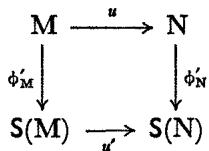
\includegraphics[keepaspectratio]{images/part003_0f38c769.jpg}}

is commutative. Moreover, \(u'\) is a graded algebra homomorphism.

The existence and uniqueness of \(u'\) follow from no. 1, Proposition 2 applied to the commutative algebra \(\mathbf{S}(\mathbf{N})\) and \(f = \phi_{\mathbf{N}}' \circ u: \mathbf{M} \to \mathbf{S}(\mathbf{N})\) ; as

\[
f (\mathbf {M}) \subset \mathbf {S} ^ {1} (\mathbf {N}) = \mathbf {N},
\]

the fact that \(u'\) is a graded algebra homomorphism follows from no. 1, Remark 1.

The homomorphism \(u'\) of Proposition 3 will henceforth be denoted by \(S(u)\) . If \(P\) is an A-module and \(v: N \to P\) an A-linear mapping, then

\[
\mathbf {S} (v \circ u) = \mathbf {S} (v) \circ \mathbf {S} (u)\tag{3}
\]

for \(\mathbf{S}(v) \circ \mathbf{S}(u)\) is an algebra homomorphism rendering commutative the diagram

\pandocbounded{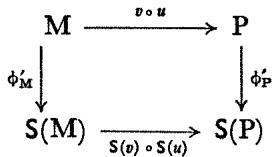
\includegraphics[keepaspectratio]{images/part003_67e6d402.jpg}}

As \(\mathbf{S}(\mathbf{M})\) contains \(\mathbf{M} = \mathbf{S}^1 (\mathbf{M})\) , \(\mathbf{S}(u)\) is sometimes called the canonical extension of \(u\) to \(\mathbf{S}(\mathbf{M})\) . The restriction \(\mathbf{S}^n (u): \mathbf{S}^n (\mathbf{M}) \to \mathbf{S}^n (\mathbf{N})\) is such that

\[
\mathsf {S} ^ {n} (u) \left(x _ {1} x _ {2} \dots x _ {n}\right) = u \left(x _ {1}\right) u \left(x _ {2}\right) \dots u \left(x _ {n}\right)
\]

where the \(x_{i} \in M\) , since \(\mathbf{S}(u)\) is an algebra homomorphism and \(\mathbf{S}^{1}(u) = u\) ; the restriction \(\mathbf{S}^{0}(u)\) to A is the identity mapping. Note that \(\mathbf{S}^{n}(u)\) can be obtained from \(\mathbf{T}^{n}(u): \mathbf{T}^{n}(\mathbf{M}) \to \mathbf{T}^{n}(\mathbf{N})\) by passing to the quotients.

PROPOSITION 4. If \(u: \mathbf{M} \to \mathbf{N}\) is a surjective A-linear mapping, the homomorphism \(\mathbf{S}(u): \mathbf{S}(\mathbf{M}) \to \mathbf{S}(\mathbf{N})\) is surjective and its kernel is the ideal of \(\mathbf{S}(\mathbf{M})\) generated by the kernel \(\mathbf{P} \subset \mathbf{M} \subset \mathbf{S}(\mathbf{M})\) of \(u\) .

We write \(v = \mathsf{T}(u) \colon \mathsf{T}(\mathbf{M}) \to \mathsf{T}(\mathbf{N})\) ; we know (§ 5, no. 2, Proposition 3) that \(v\) is surjective and hence it follows from the definitions that \(v(\mathfrak{J}_{\mathbf{M}}') = \mathfrak{J}_{\mathbf{N}}'\) ; if \(\Re\) is the kernel of \(v\) , then \(v^{-1}(\mathfrak{J}_{\mathbf{N}}') = \Re + \mathfrak{J}_{\mathbf{M}}'\) . As \(\mathsf{S}(u) \colon \mathsf{T}(\mathbf{M}) / \mathfrak{J}_{\mathbf{M}}' \to \mathsf{T}(\mathbf{N}) / \mathfrak{J}_{\mathbf{N}}'\) is derived from \(v\) by passing to the quotients, it is a surjective homomorphism whose kernel is \(\Re' = (\Re + \mathfrak{J}_{\mathbf{M}}') / \mathfrak{J}_{\mathbf{M}}'\) . As \(\Re\) is generated by the kernel \(\mathbf{P}\) of \(u\) (§ 5, no. 2), so is \(\Re'\) .

If \(u: \mathbf{M} \to \mathbf{N}\) is an injective linear mapping, it is not always true that \(\mathbf{S}(\mathbf{u})\) is an injective mapping (Exercise 1). However it is so when \(u\) is an injection such that \(u(\mathbf{M})\) is a direct factor in \(\mathbf{N}\) and then the image of \(\mathbf{S}(u)\) (isomorphic to \(\mathbf{S}(\mathbf{M})\) ) is a direct factor of \(\mathbf{S}(\mathbf{N})\) ; the proof is the same as that for the analogous assertions for \(\mathbf{T}(u)\) ( \(\S 5\) , no. 2) replacing \(\mathbf{T}\) by \(\mathbf{S}\) .

PROPOSITION 5. Let N and P be two submodules of an A-module M such that their sum \(N + P\) is a direct factor in M and their intersection \(N \cap P\) is a direct factor in N and in P. Then the homomorphisms \(\mathsf{S}(\mathsf{N}) \to \mathsf{S}(\mathsf{M}), \mathsf{S}(\mathsf{P}) \to \mathsf{S}(\mathsf{M})\) and

\[
\mathbf {S} (\mathbf {N} \cap \mathbf {P}) \rightarrow \mathbf {S} (\mathbf {M}),
\]

canonical extensions of the canonical injections, are injective; if \(\mathbf{S}(\mathbf{N})\) , \(\mathbf{S}(\mathbf{P})\) and \(\mathbf{S}(\mathbf{N} \cap \mathbf{P})\) are identified with subalgebras of \(\mathbf{S}(\mathbf{M})\) by means of these homomorphisms, then

\[
\mathbf {S} (\mathbf {N} \cap \mathbf {P}) = \mathbf {S} (\mathbf {N}) \cap \mathbf {S} (\mathbf {P}).\tag{4}
\]

The proof reduces to that of § 5, no. 2, Proposition 4 replacing T by S throughout. The hypotheses of Proposition 5 always hold for arbitrary submodules N, P of M when A is a field.

COROLLARY. Let K be a commutative field and M a vector space over K. For every element \(z \in \mathbb{S}(\mathbf{M})\) there exists a smallest vector space N of M such that \(z \in \mathbb{S}(\mathbf{N})\) and N is finite-dimensional.

The proof is derived from that of § 5, no. 2, Corollary to Proposition 4 replacing T by S throughout.

N is called the vector subspace of M associated with z.

\subsection{n-th SYMMETRIC POWER OF A MODULE AND SYMMETRIC MULTI-LINEAR MAPPINGS}

Let X, Y be two sets and n an integer \(\geqslant1\) . A symmetric mapping of \(X^{n}\) into Y is any mapping \(f: X^{n} \to Y\) such that, for every permutation \(\sigma \in S_{n}\) and every element \((x_{i}) \in X^{n}\) ,

\[
f (x _ {\sigma (1)}, x _ {\sigma (2)}, \dots , x _ {\sigma (n)}) = f (x _ {1}, x _ {2}, \dots , x _ {n}).\tag{5}
\]

As the transpositions which exchange two consecutive integers generate the group \(\mathfrak{S}_n\) (I, § 5, no. 7), it suffices that condition (5) hold when \(\sigma\) is such a transposition.

When Y is a module over a commutative ring A, clearly the set of symmetric mappings of \(X^{n}\) into Y is a submodule of the A-module \(Y^{X^{n}}\) of all mappings of \(X^{n}\) into Y.

PROPOSITION 6. Let A be a commutative ring and M and N two A-modules. If with every A-linear mapping \(g: \mathbf{S}^n(\mathbf{M}) \to \mathbf{N} (n \geqslant 1)\) is associated the n-linear mapping

\[
\left(x _ {1}, x _ {2}, \dots , x _ {n}\right) \mapsto g \left(x _ {1} x _ {2} \dots x _ {n}\right)\tag{6}
\]

(where on the right-hand side the product is taken in the algebra \(\mathbf{S}(\mathbf{M})\) ), a bijective A-linear mapping is obtained of the A-module \(\operatorname{Hom}_{\mathbf{A}}(\mathbf{S}^{n}(\mathbf{M}), \mathbf{N})\) onto the A-module of symmetric \(n\) -linear mappings of \(\mathbf{M}^{n}\) into \(\mathbf{N}\) .

Recall (II, §3, no. 9) that there is a canonical bijection of the A-module \(\operatorname{Hom}_{\mathbf{A}}(\mathbb{T}^{n}(\mathbf{M}), \mathbf{N})\) onto the A-module \(\mathcal{L}_{n}(\mathbf{M}, \ldots, \mathbf{M}; \mathbf{N})\) of all \(n\) -linear mappings of \(\mathbf{M}^{n}\) into \(\mathbf{N}\) obtained by associating with every A-linear mapping \(f: \mathbb{T}^{n}(\mathbf{M}) \to \mathbf{N}\) the \(n\) -linear mapping

\[
\bar {f} \colon (x _ {1}, x _ {2}, \dots , x _ {n}) \mapsto f (x _ {1} \otimes x _ {2} \otimes \dots \otimes x _ {n}).\tag{7}
\]

On the other hand, the A-linear mappings \(g \colon \mathbb{S}^n(\mathbf{M}) \to \mathbf{N}\) are in one-to-one correspondence with the A-linear mappings \(f \colon \mathbb{T}^n(\mathbf{M}) \to \mathbf{N}\) such that \(f\) is zero on \(\mathfrak{J}_n'\) , by associating with \(g\) the mapping \(f = g \circ p_n\) , where

\[
p _ {n} \colon \mathbf {T} ^ {n} (\mathbf {M}) \rightarrow \mathbf {S} ^ {n} (\mathbf {M}) = \mathbf {T} ^ {n} (\mathbf {M}) / \mathfrak {J} _ {n} ^ {\prime}
\]

is the canonical homomorphism (II, § 2, no. 1, Theorem 1). But as \(\mathfrak{J}_n'\) is a linear combination of elements of the form

\[
\left(u _ {1} \otimes u _ {2} \otimes \dots \otimes u _ {p}\right) \otimes (x \otimes y - y \otimes x) \otimes \left(v _ {1} \otimes \dots \otimes v _ {n - p - 2}\right)
\]

\((x, y, u_{i}, v_{j} \text{ in } \mathbf{M})\) , to say that the function f is of the form \(g \circ p_{n}\) means that the corresponding n-linear function \(\bar{f}\) satisfies the relation

\[
\bar {f} (u _ {1}, \dots , u _ {p}, x, y, v _ {1}, \dots , v _ {n - p - 2}) = \bar {f} (u _ {1}, \dots , u _ {p}, y, x, v _ {1}, \dots , v _ {n - p - 2});
\]

in other words, by what has been seen above, this means that \(\bar{f}\) is symmetric; whence the proposition, taking account of the fact that

\[
p _ {n} (x _ {1} \otimes x _ {2} \otimes \dots \otimes x _ {n}) = x _ {1} x _ {2} \dots x _ {n}
\]

with the \(x_{i} \in M\) .

The A-module \(\mathbf{S}^{n}(\mathbf{M})\) is called the n-th symmetric power of M. For every A-module homomorphism \(u: M \to N\) , the mapping \(\mathbf{S}^{n}(u): \mathbf{S}^{n}(\mathbf{M}) \to \mathbf{S}^{n}(\mathbf{N})\) which coincides with \(\mathbf{S}(u)\) on \(\mathbf{S}^{n}(\mathbf{M})\) is called the n-th symmetric power of u.

Remark. Let \(\sigma\) be a permutation in \(\mathfrak{S}_n\) ; as the mapping

\[
\left(x _ {1}, x _ {2}, \dots , x _ {n}\right) \mapsto x _ {\sigma^ {- 1} (1)} \otimes x _ {\sigma^ {- 1} (2)} \otimes \dots \otimes x _ {\sigma^ {- 1} (n)}
\]

of \(\mathbf{M}^n\) into \(\mathbf{T}^n (\mathbf{M})\) is A-multilinear, it may be written uniquely as

\[
(x _ {1}, \dots , x _ {n}) \mapsto u _ {\sigma} (x _ {1} \otimes x _ {2} \otimes \dots \otimes x _ {n}),
\]

where \(u_{\sigma}\) is an endomorphism of the A-module \(\mathsf{T}^n(\mathbf{M})\) , also denoted by \(z \mapsto \sigma. z\) . Clearly, if \(\sigma\) is the identity element of \(\mathfrak{S}_n\) , \(u_{\sigma}\) is the identity; on the other hand, writing \(y_i = x_{\sigma^{-1}(i)}\) , we obtain, for every permutation \(\tau \in \mathfrak{S}_n, y_{\tau^{-1}(i)} = x_{\sigma^{-1}(\tau^{-1}(i))}\) and hence \(\tau. (\sigma. z) = (\tau \sigma). z\) ; in other words, the A-module \(\mathsf{T}^n(\mathbf{M})\) is a left \(\mathfrak{S}_n\text{-set}\) under the operation \((\sigma, z) \mapsto \sigma. z\) (I, § 5, no. 1). The elements of \(\mathsf{T}^n(\mathbf{M})\) such that \(\sigma. z = z\) for all \(\sigma \in \mathfrak{S}_n\) are called (contravariant) symmetric tensors of order \(n\) ; they form a sub-A-module \(\mathsf{S}_n'(\mathbf{M})\) of \(\mathsf{T}^n(\mathbf{M})\) .

For all \(z \in \mathbf{T}^n(\mathbf{M})\) , we write \(s.z = \sum_{\sigma \in \mathfrak{S}_n} \sigma.z\) and call \(s.z\) the symmetrization of the tensor \(z\) ; clearly \(s.z\) is a symmetric tensor and therefore \(z \mapsto s.z\) is an endomorphism of \(\mathbf{T}^n(\mathbf{M})\) whose image \(\mathbf{S}_n''(\mathbf{M})\) is contained in \(\mathbf{S}_n'(\mathbf{M})\) ; in general, \(\mathbf{S}_n''(\mathbf{M}) \neq \mathbf{S}_n'( \mathbf{M})\) (Exercise 5). If \(z\) is a symmetric tensor, then \(s.z = n!z\) ; it follows that when \(n!\) is invertible in \(\mathbf{A}\) , the endomorphism \(z \mapsto (n!)^{-1}s.z\) is a projector of \(\mathbf{T}^n(\mathbf{M})\) (II, § 1, no. 8), whose image is \(\mathbf{S}_n'(\mathbf{M}) = \mathbf{S}_n''(\mathbf{M})\) ; moreover the kernel on this projector is just \(\mathfrak{J}_n'\) . For, obviously \(\sigma(\mathfrak{J}_n') \subset \mathfrak{J}_n'\) for all \(\sigma \in \mathfrak{S}_n\) and \(\mathfrak{J}_n'\) is by definition generated by the tensors \(z - \rho.z\) , where \(\rho\) is a transposition exchanging two consecutive numbers in {[}1, n{]}; also, if \(\sigma, \tau\) are two permutations in \(\mathfrak{S}_n\) , then \(z - (\sigma\tau).z = z - \sigma.z + \sigma.(z - \tau.z)\) , whence it follows (since every permutation in \(\mathfrak{S}_n\) is a product of transpositions exchanging two consecutive numbers) that \(z - \sigma.z \in \mathfrak{J}_n'\) for all \(z \in \mathbf{T}^n(\mathbf{M})\) and \(\sigma \in \mathfrak{S}_n\) . Therefore (always supposing that \(n!\) is invertible in \(\mathbf{A}\) ), it is seen that \(z - (n!)^{-1}s.z = \sum_{\sigma \in \mathfrak{S}_n}(n!)^{-1}(z - \sigma.z) \in \mathfrak{J}_n'\) for all \(z \in \mathbf{T}^n(\mathbf{M})\) , which proves our assertion.

When \(n!\) is invertible in A, the submodules \(S_n'(M)\) and \(\mathfrak{S}_n'\) of \(T^n(M)\) are therefore supplementary and the restriction to \(S_n'(M)\) of the canonical homomorphism \(T^n(M) \to S^n(M) = T^n(M)/\mathfrak{J}_n'\) is an A-module isomorphism, which allows us in the case envisaged to identify symmetric tensors of order \(n\) with the elements of the \(n\) -th symmetric power of M. Note however that this identification is not compatible with multiplication, the product (in \(T(M)\) ) of two symmetric tensors not being symmetric in general and not therefore having as image in \(S(M)\) the product of the images of the symmetric tensors considered.

\subsection{EXTENSION OF THE RING OF SCALARS}

Let A, A' be two commutative rings, \(\rho: A \to A'\) a ring homomorphism, M an A-module, M' an A'-module and \(f: M \to M'\) an A-homomorphism (relative to \(\rho\) ) of M into M'. The composite mapping \(M \xrightarrow{f} M' \xrightarrow{\phi_{M'}'} S_{A'}(M')\) is an A-linear mapping of M into the commutative algebra \(\rho_*(S_A(M'))\) ; then there exists no. 1, Proposition 2) one and only one A-homomorphism of algebras \(f': S_A(M) \to S_{A'}(M')\) rendering commutative the diagram

\[
\begin{array}{c} \mathrm{M} \xrightarrow {f} \mathrm{M} ^ {\prime} \\ \phi_ {\mathrm{M}} ^ {\prime} \Biggl \downarrow \\ \mathrm{S} _ {\mathrm{A}} (\mathrm{M}) \xrightarrow [ f ^ {\prime} ]{} \mathrm{S} _ {\mathrm{A} ^ {\prime}} (\mathrm{M} ^ {\prime}) \end{array}\tag{8}
\]

It follows immediately that if \(\sigma: A' \to A''\) is another ring homomorphism, \(M''\) an \(A''\) -module, \(g: M' \to M''\) an \(A'\) -homomorphism (relative to \(\sigma\) ) and \(g': S_{A'}(M') \to S_{A''}(M'')\) the corresponding \(A'\) -homomorphism of algebras, then the composite \(A\) -homomorphism of algebras

\[
\mathrm{S} _ {\mathrm{A}} (\mathrm{M}) \xrightarrow {f ^ {\prime}} \mathrm{S} _ {\mathrm{A} ^ {\prime}} \left(\mathrm{M} ^ {\prime}\right) \xrightarrow {g ^ {\prime}} \mathrm{S} _ {\mathrm{A} ^ {\prime \prime}} \left(\mathrm{M} ^ {\prime \prime}\right)\tag{9}
\]

corresponds to the composite A-homomorphism \(g \circ f: \mathbf{M} \to \mathbf{M}''\) (relative to \(\sigma \circ \rho\) ).

PROPOSITION 7. Let A, B be two commutative rings, \(\rho: \mathbf{A} \to \mathbf{B}\) a ring homomorphism and M an A-module. The canonical extension

\[
\psi \colon \mathbf {S} _ {\mathbf {B}} (\mathbf {B} \otimes_ {\mathbf {A}} \mathbf {M}) \rightarrow \mathbf {B} \otimes_ {\mathbf {A}} \mathbf {S} _ {\mathbf {A}} (\mathbf {M})
\]

of the B-linear mapping \(1_{B} \otimes \phi_{M}'\) : \(B \otimes_{A} M \to B \otimes_{A} S_{A}(M)\) is a graded B-algebra isomorphism.

The proof is derived from that of § 5, no. 3, Proposition 5 replacing T by S and \(\phi_{\mathbf{M}}\) by \(\phi_{\mathbf{M}}^{\prime}\) .

\subsection{DIRECT LIMIT OF SYMMETRIC ALGEBRAS}

Let \((\mathbf{A}_{\alpha},\phi_{\beta \alpha})\) be a directed direct system of commutative rings, \((\mathbf{M}_{\alpha},f_{\beta \alpha})\) a direct system of \(\mathbf{A}_{\alpha}\) -modules, \(\mathbf{A} = \varinjlim \mathbf{A}_{\alpha}\) and \(\mathbf{M} = \varinjlim \mathbf{M}_{\alpha}\) . For \(\alpha \leqslant \beta\) , we derive canonically from the \(\mathbf{A}_{\alpha}\) -homomorphism \(f_{\beta \alpha}: \mathbf{M}_{\alpha} \to \mathbf{M}_{\beta}\) an \(\mathbf{A}_{\alpha}\) -algebra homomorphism (no. 4, formula (8)) \(f_{\beta \alpha}': \mathbf{S}_{\mathbf{A}_{\alpha}}(\mathbf{M}_{\alpha}) \to \mathbf{S}_{\mathbf{A}_{\beta}}(\mathbf{M}_{\beta})\) and it follows from (9) (no. 4) that \((\mathbf{S}_{\mathbf{A}_{\alpha}}(\mathbf{M}_{\alpha}), f_{\beta \alpha}')\) is a direct system of \(\mathbf{A}_{\alpha}\) -algebras. On the other hand, let \(f_{\alpha}: \mathbf{M}_{\alpha} \to \mathbf{M}\) be the canonical A-homomorphism; we derive (no. 4, formula (8)) an \(\mathbf{A}_{\alpha}\) -algebra homomorphism

\[
f _ {\alpha} ^ {\prime}: \mathrm{S} _ {\mathrm{A} _ {\alpha}} (\mathbf {M} _ {\alpha}) \rightarrow \mathrm{S} _ {\mathrm{A}} (\mathbf {M})
\]

and it also follows from (9) that the \(f_{\alpha}'\) constitute a direct system of \(A_{\alpha}\) -homomorphisms.

PROPOSITION 8. The A-homomorphism \(f' = \varinjlim f_{\alpha}' \colon \varinjlim S_{A_{\alpha}}(M_{\alpha}) \to S_{A}(M)\) is a graded algebra isomorphism.

The proof is the same as that of § 5, no. 5, Proposition 6 replacing throughout T by S and \(\phi\) by \(\phi'\) and taking account of the fact that a direct limit of commutative algebras is commutative.

\subsection{SYMMETRIC ALGEBRA OF A DIRECT SUM. SYMMETRIC ALGEBRA OF A FREE MODULE. SYMMETRIC ALGEBRA OF A GRADED MODULE}

Let A be a commutative ring, \(M = \bigoplus_{\lambda \in L} M_{\lambda}\) the direct sum of a family of A-modules and \(j_{\lambda}: M_{\lambda} \to M\) the canonical injection; we derive an A-homomorphism of algebras \(\mathsf{S}(j_{\lambda}): \mathsf{S}(\mathsf{M}_{\lambda}) \to \mathsf{S}(\mathsf{M})\) . Since \(\mathsf{S}(\mathsf{M})\) is commutative, Proposition 8 of §4, no. 5, can be applied to the homomorphisms \(\mathsf{S}(j_{\lambda})\) and there therefore exists a unique algebra homomorphism

\[
g \colon \bigotimes_ {\lambda \in L} \mathbf {S} (\mathbf {M} _ {\lambda}) \rightarrow \mathbf {S} (\mathbf {M})\tag{10}
\]

(also denoted by \(g_{\mathbf{M}}\) ) such that \(\mathbf{S}(j_{\lambda}) = g \circ f_{\lambda}\) for all \(\lambda \in \mathbf{L}\) , where

\[
f _ {\lambda} \colon \mathbf {S} (\mathbf {M} _ {\lambda}) \rightarrow \bigotimes_ {\lambda \in \mathbf {L}} \mathbf {S} (\mathbf {M} _ {\lambda})
\]

denotes the canonical homomorphism.

PROPOSITION 9. The canonical homomorphism \(g\) (formula (10)) is a graded algebra isomorphism (cf.~§4, no. 8, Remark 1).

To prove that \(g\) is bijective, we define an algebra homomorphism

\begin{enumerate}
\def\labelenumi{(\arabic{enumi})}
\setcounter{enumi}{10}
\tightlist
\item
\end{enumerate}

\[
h \colon \mathbf {S} (\mathbf {M}) \rightarrow \bigotimes_ {\lambda \in L} \mathbf {S} (\mathbf {M} _ {\lambda})
\]

such that \(g \circ h\) and \(h \circ g\) are respectively the identity mappings on \(\mathbf{S}(\mathbf{M})\) and \(\bigotimes_{\lambda \in \mathbf{L}} \mathbf{S}(\mathbf{M}_{\lambda})\) . For each \(\lambda \in \mathbf{L}\) , let \(u_{\lambda}\) be the composite linear mapping

\[
\mathbf {M} _ {\lambda} \xrightarrow {\phi_ {\mathrm{M} _ {\lambda}} ^ {\prime}} \mathbf {S} (\mathbf {M} _ {\lambda}) \xrightarrow {f _ {\lambda}} \bigotimes_ {\lambda \in L} \mathbf {S} (\mathbf {M} _ {\lambda}).
\]

There exists one and only one A-linear mapping \(u: \mathbf{M} \to \bigotimes_{\lambda \in L} \mathbf{S}(\mathbf{M}_{\lambda})\) such that \(u \circ j_{\lambda} = u_{\lambda}\) for all \(\lambda \in L\) . As the \(\mathbf{S}(\mathbf{M}_{\lambda})\) are commutative, so is their tensor product (§ 4, no. 5) and hence (no. 1, Proposition 2) there exists a unique algebra homomorphism \(h: \mathbf{S}(\mathbf{M}) \to \bigotimes_{\lambda \in L} \mathbf{S}(\mathbf{M}_{\lambda})\) such that \(h \circ \phi_{\mathbf{M}}' = u\) ; on the other hand, it is immediate that \(u(\mathbf{M})\) is contained in the submodule of elements of degree 1 of the graded algebra \(\bigotimes_{\lambda \in L} \mathbf{S}(\mathbf{M}_{\lambda})\) and hence \(h\) is a graded algebra homomorphism. For \(x_{\lambda} \in \mathbf{M}_{\lambda}\) ,

\[
h \left(g \left(u _ {\lambda} \left(x _ {\lambda}\right)\right)\right) = h \left(g \left(f _ {\lambda} \left(\phi_ {M _ {\lambda}} ^ {\prime} \left(x _ {\lambda}\right)\right)\right)\right) = h \left(S \left(j _ {\lambda}\right) \left(\phi_ {M _ {\lambda}} ^ {\prime} \left(x _ {\lambda}\right)\right)\right) = h \left(\phi_ {M} ^ {\prime} \left(j _ {\lambda} \left(x _ {\lambda}\right)\right)\right) = u _ {\lambda} \left(x _ {\lambda}\right);
\]

as the \(u_{\lambda}(x_{\lambda})\) generate the algebra \(\bigotimes_{\lambda \in L} S(M_{\lambda})\) (§ 4, no. 5, Proposition 8), \(h \circ g\) is certainly the identity mapping. Similarly,

\[
g \left(h \left(\phi_ {\mathrm{M}} ^ {\prime} \left(j _ {\lambda} \left(x _ {\lambda}\right)\right)\right)\right) = g \left(u _ {\lambda} \left(x _ {\lambda}\right)\right) = g \left(f _ {\lambda} \left(\phi_ {\mathrm{M} _ {\lambda}} ^ {\prime} \left(x _ {\lambda}\right)\right)\right) = \mathrm{S} \left(j _ {\lambda}\right) \left(\phi_ {\mathrm{M} _ {\lambda}} ^ {\prime} \left(x _ {\lambda}\right)\right) = \phi_ {\mathrm{M}} ^ {\prime} \left(j _ {\lambda} \left(x _ {\lambda}\right)\right)
\]

and, as the elements \(\phi_{\mathbf{M}}^{\prime}(j_{\lambda}(x_{\lambda}))\) generate the algebra \(\mathbf{S}(\mathbf{M})\) , \(g \circ h\) is certainly the identity mapping.

Remark (1) Let \(\mathbf{N} = \bigoplus_{\lambda \in L} \mathbf{N}_{\lambda}\) be the direct sum of another family of A-modules with \(L\) as indexing set and, for all \(\lambda \in L\) , let \(v_{\lambda}: \mathbf{M}_{\lambda} \to \mathbf{N}_{\lambda}\) be an A-linear mapping, whence there is an A-linear mapping \(v = \bigoplus_{\lambda} v_{\lambda}: \mathbf{M} \to \mathbf{N}\) (II, § 1, no. 6, Proposition 6). Then the diagram

\[
\begin{array}{c} \bigotimes_ {\lambda \in L} S (M _ {\lambda}) \xrightarrow {g _ {M}} S (M) \\ \bigoplus_ {\lambda \in L} S (v _ {\lambda}) \Biggl \downarrow \qquad \qquad \qquad \qquad \qquad \qquad \qquad \qquad \qquad \Biggl \downarrow S (v) \\ \bigotimes_ {\lambda \in L} S (N _ {\lambda}) \xrightarrow {g _ {N}} S (N) \end{array}
\]

is commutative, as follows from the definitions (§ 4, no. 5, Corollary to Proposition 8).

The sub-A-module of \(\bigotimes_{\lambda \in L} \mathbf{S}(\mathbf{M}_{\lambda})\) with which \(\mathbf{S}^n(\mathbf{M})\) is identified by means of the isomorphism \(g\) can be described more precisely. For every finite subset \(J\) of \(L\) , we write \(\mathbf{E}_J = \bigotimes_{\lambda \in J} \mathbf{S}(\mathbf{M}_{\lambda})\) , so that \(\bigotimes_{\lambda \in L} \mathbf{S}(\mathbf{M}_{\lambda}) = \varinjlim \mathbf{E}_J\) relative to the directed set \(\mathfrak{F}(\mathrm{L})\) of finite subsets of \(\mathbf{L}\) , by definition (§ 4, no. 5). For every family \(\nu = (n_{\lambda}) \in \mathbf{N}^{(\mathbf{L})}\) (thus having finite support) such that \(\sum_{\lambda \in \mathbf{L}} n_{\lambda} = n\) and every finite subset \(\mathbf{J}\) of \(\mathbf{L}\) containing the support of the family \(\nu\) , we write

\[
\mathbf {S} ^ {\mathrm{J}, \nu} (\mathbf {M}) = \bigotimes_ {\lambda \in J} \mathbf {S} ^ {n _ {\lambda}} (\mathbf {M} _ {\lambda})\tag{12}
\]

so that the submodule \(E_{J,n}\) of elements of degree n in \(E_{J}\) is the direct sum of the \(S^{J,v}(M)\) over all the families v of support contained in J and such that \(\sum_{\lambda\in L}n_{\lambda}=n\) ( \(\S4\) , no. 7, Proposition 10 and \(\S4\) , no. 8). As a convention we write \(S^{J,v}(M)=\{0\}\) for the families v whose support is not contained in J; then \(E_{J,n}\) can also be called the direct sum of all the \(S^{J,v}(M)\) , where v runs through the set \(H_{n}\) of all families \(v=(n_{\lambda})_{\lambda\in L}\) such that \(\sum_{\lambda\in L}n_{\lambda}=n\) . Since \(S^{0}(M_{\lambda})\) is identified with A, clearly also, for two finite subsets \(J\subset J'\) of L and a family v of support contained in J, the canonical mapping \(S^{J,v}(M)\to S^{J',v}(M)\) (restriction of the canonical mapping \(E_{J}\to E_{J'}\) to \(S^{J,v}(M)\) ) is bijective. If we write, for all \(v\in H_{n}\) ,

\[
\mathbf {S} ^ {\nu} (\mathbf {M}) = \varinjlim \mathbf {S} ^ {\mathrm{J}, \nu} (\mathbf {M})\tag{13}
\]

it is seen that, taking account of II, § 6, no. 2, Proposition 5:

COROLLARY. The A-module \(\mathbf{S}^n (\mathbf{M})\) is the image under isomorphism (10) of the submodule of \(\bigotimes_{\lambda \in \mathbf{L}}\mathbf{S}(\mathbf{M}_{\lambda})\) the direct sum of the submodules \(\mathbf{S}^{\nu}(\mathbf{M})\) for all the families \(\nu = (n_{\lambda})\in \mathbf{N}^{(L)}\) such that \(\sum_{\lambda \in \mathbf{L}}n_{\lambda} = n\) ; if \(\mathbf{J}\) is the support of \(\nu\) , \(\mathbf{S}^{\nu}(\mathbf{M})\) is canonically isomorphic to \(\bigotimes_{\lambda \in \mathbf{J}}\mathrm{S}^{n_{\lambda}}(\mathbf{M}_{\lambda})\) .

In general \(\mathbf{S}^{\nu}(\mathbf{M}),\bigotimes_{\lambda \in J}\mathbf{S}^{n_{\lambda}}(\mathbf{M}_{\lambda})\) and their image in \(\mathbf{S}^n (\mathbf{M})\) are identified.

THEOREM 1. Let A be a commutative ring and M a free A-module with basis \((e_{\lambda})_{\lambda \in L}\) . For every mapping \(\alpha: \mathbf{L} \to \mathbf{N}\) of finite support, we write

\[
e ^ {\alpha} = \prod_ {\lambda \in L} e _ {\lambda} ^ {\alpha (\lambda)}\tag{14}
\]

(product in the commutative algebra \(\mathbf{S}(\mathbf{M})\) ). Then, when \(\alpha\) runs through the set \(\mathbf{N}^{(L)}\) of mappings of \(\mathbf{L}\) into \(\mathbf{N}\) , of finite support, the \(e^{\alpha}\) form a basis of the A-module \(\mathbf{S}(\mathbf{M})\) .

As M is the direct sum of the \(M_{\lambda} = Ae_{\lambda}\) , it suffices to prove the theorem when L is reduced to a single element and then apply Proposition 9. But when M = Ae (e a free element), then \(x \otimes y - y \otimes x = 0\) for all x, y in M; the ideal \(J'\) is therefore zero, whence \(\mathsf{T}(\mathsf{A}e) = \mathsf{S}(\mathsf{A}e)\) and the theorem then follows from §5, no. 5, Theorem 1.

The multiplication table of the basis (14) is given by

\[
e ^ {\alpha} e ^ {\beta} = e ^ {\alpha + \beta}\tag{15}
\]

where \(\alpha + \beta\) is the mapping \(\lambda \mapsto \alpha(\lambda) + \beta(\lambda)\) of L into N. In other words, the basis \((e^{\alpha})\) of S(M), with the multiplicative law (15), is canonically isomorphic to the free commutative monoid \(\mathbf{N}^{(L)}\) derived from L; it follows (§ 2, no. 9) that the symmetric algebra S(M) of a free module M with basis whose indexing set is L, is canonically isomorphic to the polynomial algebra A{[}(X \(_{\lambda}\) ) \(_{\lambda \in L}\) {]}, the canonical isomorphism being obtained by mapping \(e_{\lambda}\) to X \(_{\lambda}\) . In particular (§ 2, no. 7, Proposition 7), for every mapping \(f\colon\) L \(\to\) E of L into a commutative A-algebra E, there exists one and only one A-algebra homomorphism \(\bar{f}\colon\) S(M) \(\to\) E such that \(\bar{f}(e_{\lambda}) = f(\lambda)\) .

Remark (2). The above results can equally well be obtained as a consequence of the universal properties of polynomial algebras and symmetric algebras, taking account of II, § 1, no. 11, Corollary 3 to Proposition 17.

COROLLARY. If M is a projective A-module, S(M) is a projective A-module.

The proof is the same as that for § 5, no. 5, Corollary to Theorem 1, replacing T by S.

PROPOSITION 10. Let \(\Delta\) be a commutative monoid, \(\mathbf{M}\) a graded A-module of type \(\Delta\) and \((\mathbf{M}_{\alpha})_{\alpha \in \Delta}\) its graduation. For every ordered pair \((\alpha, n) \in \Delta \times \mathbf{N}\) , let \(\mathbf{S}^{\alpha, n}(\mathbf{M})\) be the submodule of \(\mathbf{S}^n(\mathbf{M})\) the direct sum of the submodules \(\bigotimes_{\lambda \in J} \mathbf{S}^{n_{\lambda}}(\mathbf{M}_{\alpha_{\lambda}})\) , where \((n_{\lambda})_{\lambda \in L}\) runs through the set of families of integers \(\geqslant 0\) such that \(\sum_{\lambda \in L} n_{\lambda} = n, J\) is its support and, for each \((n_{\lambda})\) , \((\alpha_{\lambda})_{\lambda \in J}\) runs through the set of families of \(\Delta^J\) such that \(\sum_{\lambda \in J} \alpha_{\lambda} = \alpha\) . Then \((\mathbf{S}^{\alpha, n}(\mathbf{M}))_{(\alpha, n) \in \Delta \times \mathbf{N}}\) is the only graduation of type \(\Delta \times \mathbf{N}\) compatible with the algebra structure on \(\mathbf{S}(\mathbf{M})\) and which induces on \(\mathbf{M} = \mathbf{S}^1(\mathbf{M})\) the given graduation.

The fact that \(\mathbf{S}(\mathbf{M})\) is the direct sum of the \(\mathbf{S}^{\alpha,n}(\mathbf{M})\) follows from the Corollary to Proposition 9; the rest of the proof is identical with the end of the proof of §5, no. 5, Proposition 7.

Suppose more particularly that \(\Delta = \mathbf{Z}\) and let \(\mathbb{S}(\mathbf{M})\) be given the total graduation (of type \(\mathbf{Z}\) ) (II, §11, no. 1) corresponding to the graduation of type \(\mathbf{Z} \times \mathbf{N}\) (and hence also of type \(\mathbf{Z} \times \mathbf{Z}\) ) defined above; the homogeneous elements of degree \(n \in \mathbf{Z}\) under this graduation are therefore those of the direct sum of the \(\mathbb{S}^{q, m}(\mathbf{M})\) for \(q + m = n\) . Let \(f\) be a homogeneous linear mapping of degree 0 of the graded A-module \(\mathbf{M}\) into a commutative graded A-algebra \(\mathbf{F}\) of type \(\mathbf{Z}\) ; then the algebra homomorphism \(g: \mathbb{S}(\mathbf{M}) \to \mathbf{F}\) such that \(f = g \circ \phi_{\mathbf{M}}'\) is a homomorphism of graded algebras of type \(\mathbf{Z}\) , as follows from the formula \(g(x_1 x_2 \ldots x_n) = f(x_1) f(x_2) \ldots f(x_n)\) for homogeneous \(x_i\) in \(\mathbf{M}\) , from the hypothesis on \(f\) and from the definition of the graduation of type \(\mathbf{Z}\) on \(\mathbb{S}(\mathbf{M})\) .

\section{EXTERIOR ALGEBRAS}

\subsection{DEFINITION OF THE EXTERIOR ALGEBRA OF A MODULE}

DEFINITION 1. Let A be a commutative ring and M an A-module. The exterior algebra of M, denoted by \(\bigwedge (\mathbf{M})\) or \(\operatorname {Alt}(\mathbf{M})\) or \(\bigwedge_{\mathbf{A}}(\mathbf{M})\) , is the algebra over A the quotient of the tensor algebra \(\mathsf{T}(\mathbf{M})\) by the two-sided ideal \(\mathfrak{J}''\) (also denoted by \(\mathfrak{J}_{\mathbf{M}}''\) ) generated by the elements \(x\otimes x\) , where \(x\) runs through M.

Since the ideal \(\mathfrak{J}''\) is generated by homogeneous elements of degree 2, it is a graded ideal (II, §11, no. 3, Proposition 2); we write \(\mathfrak{J}_n'' = \mathfrak{J}'' \cap \mathsf{T}^n(\mathbf{M})\) ; the algebra \(\bigwedge(\mathbf{M})\) is therefore graded by the graduation (called canonical) consisting of the \(\bigwedge^n(\mathbf{M}) = \mathsf{T}^n(\mathbf{M}) / \mathfrak{J}_n''\) . Then \(\mathfrak{J}_0'' = \mathfrak{J}_1'' = \{0\}\) and hence \(\bigwedge^0(\mathbf{M})\) is identified with A and \(\bigwedge^1(\mathbf{M})\) with \(\mathsf{T}^1(\mathbf{M}) = \mathbf{M}\) ; in what follows we shall always make these identifications and the canonical injection \(\mathbf{M} \to \bigwedge(\mathbf{M})\) will be denoted by \(\phi''\) or \(\phi_{\mathbf{M}}''\) .

PROPOSITION 1. Let E be an A-algebra and \(f: \mathbf{M} \to \mathbf{E}\) an A-linear mapping such that

\[
(f (x)) ^ {2} = 0 \quad \text { for all } x \in \mathbf {M}.\tag{1}
\]

There exists one and only one A-algebra homomorphism \(g: \bigwedge(\mathbf{M}) \to \mathbf{E}\) such that \(f = g \circ \phi''\) .

In other words, \((\bigwedge (\mathbf{M}),\phi '')\) is a solution of the universal mapping problem (Set Theory, IV, § 3, no. 1), where \(\Sigma\) is the species of A-algebra structure, the \(\alpha\) -mappings being the linear mappings from the A-module M to an A-algebra satisfying (1).

The uniqueness of \(g\) follows from the fact that \(\phi''(\mathbf{M}) = \mathbf{M}\) generates \(\bigwedge (\mathbf{M})\) . To prove the existence of \(g\) , we note that by § 5, no. 1, Proposition 1 there exists an A-algebra homomorphism \(g_1: \mathsf{T}(\mathbf{M}) \to \mathbf{E}\) such that \(f = g_1 \circ \phi\) ; we need to prove that \(g_1\) is zero on the ideal \(\mathfrak{J}''\) , for then if

\[
p \colon \mathbf {T} (\mathbf {M}) \rightarrow \bigwedge (\mathbf {M}) = \mathbf {T} (\mathbf {M}) / \mathfrak {J} ^ {\prime \prime}
\]

is the canonical homomorphism, we can write \(g_1 = g \circ p\) , where \(g: \bigwedge (\mathbf{M}) \to \mathbf{E}\) is an algebra homomorphism and the conclusion will follow from the fact that \(p \circ \phi = \phi''\) . Now, the kernel of \(g_1\) is a two-sided ideal which, by virtue of (1) and the relation \(g_1 \circ \phi = f\) , contains the elements \(x \otimes x\) for \(x \in \mathbf{M}\) . This completes the proof.

Remarks. (1) Suppose that E is a graded A-algebra of type Z, of graduation \((\mathbf{E}_{n})\) , and suppose also that the linear mapping f (assumed to satisfy (1)) is such that

\[
f (\mathbf {M}) \subset \mathbf {E} _ {1}.\tag{2}
\]

Then the relation \(g(x_1x_2 \ldots x_p) = f(x_1)f(x_2) \ldots f(x_p)\) with the \(x_i \in \mathbf{M}\) shows that \(g(\bigwedge^p (\mathbf{M})) \subset \mathrm{E}_p\) for all \(p \geqslant 0\) and hence \(g\) is a graded algebra homomorphism.

\begin{enumerate}
\def\labelenumi{(\arabic{enumi})}
\setcounter{enumi}{1}
\tightlist
\item
  To avoid confusion, the product of two elements u, v of the exterior algebra \(\bigwedge(\mathbf{M})\) is usually denoted by \(u \wedge v\) and is called the exterior product of u by v. The elements of \(\bigwedge^{n}(\mathbf{M})\) are therefore the sums of elements of the form \(x_{1} \wedge x_{2} \wedge \cdots \wedge x_{n}\) with \(x_{i} \in M\) for \(1 \leqslant i \leqslant n\) and are often called n-vectors.
\end{enumerate}

\subsection{FUNCTORIAL PROPERTIES OF THE EXTERIOR ALGEBRA}

PROPOSITION 2. Let A be a commutative ring, M and N two A-modules and u: M → N an A-linear mapping. There exists one and only one A-algebra homomorphism

\[
u ^ {\prime \prime}: \bigwedge (\mathbf {M}) \rightarrow \bigwedge (\mathbf {N})
\]

such that the diagram

\pandocbounded{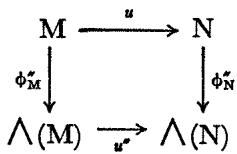
\includegraphics[keepaspectratio]{images/part003_b216bf24.jpg}}

is commutative. Moreover, \(u''\) is a graded algebra homomorphism.

The existence and uniqueness of \(u''\) follow from no. 1, Proposition 1 applied to the algebra \(\bigwedge(\mathbf{N})\) and \(f = \phi_{\mathbf{N}}'' \circ u: \mathbf{M} \to \bigwedge(\mathbf{N})\) ; for \(f(\mathbf{M}) \subset \mathbf{N}\) and hence \(f\) satisfies condition (1) by definition of \(\mathfrak{J}_{\mathbf{N}}''\) : as \(f(\mathbf{M}) \subset \bigwedge^{1}(\mathbf{N}) = \mathbf{N}\) , the fact that \(u''\) is a graded algebra homomorphism follows from Remark 1 of no. 1.

The homomorphism \(u''\) of Proposition 2 will henceforth be denoted by \(\bigwedge(u)\) . If P is an A-module and \(v: \mathbf{N} \to \mathbf{P}\) is an A-linear mapping, then

\[
\bigwedge (v \circ u) = \bigwedge (v) \circ \bigwedge (u)\tag{3}
\]

for \(\bigwedge(v) \circ \bigwedge(u)\) is an algebra homomorphism which renders commutative the diagram

\pandocbounded{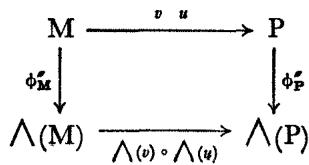
\includegraphics[keepaspectratio]{images/part003_3a522f8d.jpg}}

Since \(\bigwedge (\mathbf{M})\) contains \(\mathbf{M} = \bigwedge^{1}(\mathbf{M}),\bigwedge (u)\) is sometimes called the canonical extension of \(u\) to \(\bigwedge (\mathbf{M})\) . The restriction \(\bigwedge^n (u):\bigwedge^n (\mathbf{M})\to \bigwedge^n (\mathbf{N})\) is such that

\[
\bigwedge^ {n} (u) (x _ {1} \land x _ {2} \land \dots \land x _ {n}) = u (x _ {1}) \land u (x _ {2}) \land \dots \land u (x _ {n})\tag{4}
\]

with the \(x_{i}\in\mathbf{M}\) , since \(\bigwedge(u)\) is an algebra homomorphism and \(\bigwedge^{1}(u)=u\) ; the restriction \(\bigwedge^{0}(u)\) to A is the identity mapping. Note that \(\bigwedge^{n}(u)\) is obtained from \(\mathsf{T}^{n}(u):\mathsf{T}^{n}(\mathbf{M})\to\mathsf{T}^{n}(\mathbf{N})\) by passing to the quotients.

PROPOSITION 3. If \(u: \mathbf{M} \to \mathbf{N}\) is a surjective A-linear mapping, the homomorphism \(\bigwedge(u): \bigwedge(\mathbf{M}) \to \bigwedge(\mathbf{N})\) is surjective and its kernel is the two-sided ideal of \(\bigwedge(\mathbf{M})\) generated by the kernel \(\mathbf{P} \subset \mathbf{M} \subset \bigwedge(\mathbf{M})\) of \(u\) .

The proof is derived from that of §6, no. 2, Proposition 4, replacing S by \(\bigwedge\) and \(\mathfrak{J}'\) by \(\mathfrak{J}''\) .

If \(u: \mathbf{M} \to \mathbf{N}\) is an injective linear mapping, it is not always true that \(\bigwedge(\mathbf{u})\) is an injective mapping (§ 6, Exercise 3) (see however below no. 9, Corollary to Proposition 12). However this is so when \(u\) is an injection such that \(u(\mathbf{M})\) is a direct factor of \(\mathbf{N}\) and then the image of \(\bigwedge(u)\) (isomorphic to \(\bigwedge(\mathbf{M})\) ) is a direct factor of \(\bigwedge(\mathbf{N})\) ; the proof is the same as that for the analogous assertions for \(\mathbf{T}(u)\) (§ 5, no. 2) replacing \(\mathbf{T}\) by \(\bigwedge\) .

PROPOSITION 4. Let N and P be two submodules of an A-module M such that their sum N + P is a direct factor in M and their intersection N ∩ P is a direct factor in N and in P. Then the homomorphisms \(\bigwedge(\mathrm{N}) \to \bigwedge(\mathrm{M})\) , \(\bigwedge(\mathrm{P}) \to \bigwedge(\mathrm{M})\) and \(\bigwedge(\mathrm{N} \cap \mathrm{P}) \to \bigwedge(\mathrm{M})\) , canonical extensions of the canonical injections, are injective; if \(\bigwedge(\mathrm{N})\) , \(\bigwedge(\mathrm{P})\) and \(\bigwedge(\mathrm{N} \cap \mathrm{P})\) are identified with subalgebras of \(\bigwedge(\mathrm{M})\) by means of these homomorphisms, then

\[
\bigwedge (\mathbf {N} \cap \mathbf {P}) = \bigwedge (\mathbf {N}) \cap \bigwedge (\mathbf {P}).\tag{5}
\]

The proof is derived from that of § 5, no. 2, Proposition 4 replacing T by \(\bigwedge\) throughout. The hypotheses of Proposition 4 are always satisfied by arbitrary submodules N, P of M when A is a field.

COROLLARY. Let K be a commutative field and M a vector space over K. For every element \(z \in \bigwedge(\mathbf{M})\) , there exists a smallest vector subspace N of M such that \(z \in \bigwedge(\mathbf{N})\) and N is finite-dimensional.

The proof is deduced from that of § 5, no. 2, Corollary to Proposition 4 replacing T by \(\bigwedge\) throughout.

N is called the vector subspace of M associated with the element z of \(\bigwedge(\mathbf{M})\) .
